\documentclass{beamer}
\usetheme{Madrid}

\usepackage{textpos}
\usepackage{tikz}
\usetikzlibrary{calc}
%% Colors
\def \BLUE {blue}
\def \GREEN {green}
\def \ORANGE {orange}
\def \RED {red}
\def \VIOLET {violet}
\def \YELLOW {lime}
\usepackage{units}
\usepackage{url}

\makeatletter
\setbeamertemplate{footline}
{
  \leavevmode
  \hbox{%
  \begin{beamercolorbox}[wd=.20\paperwidth,ht=2.25ex,dp=1ex,center]{author in head/foot}%
    \usebeamerfont{author in head/foot}\insertshortauthor
  \end{beamercolorbox}%
  \begin{beamercolorbox}[wd=.30\paperwidth,ht=2.25ex,dp=1ex,center]{title in head/foot}%
    \usebeamerfont{title in head/foot}\insertshorttitle
  \end{beamercolorbox}%
  \begin{beamercolorbox}[wd=.30\paperwidth,ht=2.25ex,dp=1ex,center]{author in head/foot}%
    \usebeamerfont{author in head/foot}{Advances in Physics Seminar}
  \end{beamercolorbox}%
  \begin{beamercolorbox}[wd=.20\paperwidth,ht=2.25ex,dp=1ex,right]{date in head/foot}%
    \usebeamerfont{date in head/foot}\insertdate{}\hspace*{2em}
    \insertframenumber{} / \inserttotalframenumber\hspace*{2ex} 
  \end{beamercolorbox}}%
  \vskip0pt%
}
\makeatother

\title{Nuclear Resonance Fluorescence}
\subtitle{Basics, Applications, and Recent Advances}
\author[U. Friman-Gayer]{Udo Friman-Gayer\inst{1,2}}
\institute{
    \inst{1} Department of Physics and Astronomy, University of North Carolina at Chapel Hill, Chapel Hill, NC \\
    \inst{2} Triangle Universities Nuclear Laboratory, Duke University, Durham, NC
}
\date{Advances in Physics Seminar, 06/18/2020}

\begin{document}

\begin{frame}
    \titlepage
\end{frame}

\begin{frame}
    \frametitle{Outline}
    \tableofcontents
\end{frame}

\section{Introduction}

\subsection{'Scattering' of Photons}

\begin{frame}
    \frametitle{Interaction of Photons with Matter}
    %\def \SLIDEINRED {2}
\def \SLIDEOUTRED {3}
\def \SLIDERED {4}
\def \SLIDEGREEN {5}
\def \SLIDEBLUE {6}
\def \SLIDEVIOLET {7}

\begin{textblock}{15.}(0., -5.)
    \begin{tikzpicture}
        %%% Definitions
        %% Mathematical constants
        \def \INVERSESQRTTWO {0.7071067811865475}
        \def \NWAVEFORMSAMPLES {400}

        %% Colors
        \def \BLUE {blue}
        \def \GREEN {green}
        \def \VIOLET {violet}
        \def \RED {red}

        %% Labels
        \def \LABELLOWSTART {-1.}
        \def \LABELLOWSTOP {-2.}
        \def \LABELUPSTART {-1.}
        \def \LABELUPSTOP {-1.5}

        %% Schematic model of the nucleus
        \coordinate (NUCLEUSPOSITION) at (6., 0.);

        \def \NUCLEONRADIUS {0.3}
        \def \NUCLEONDISTANCE {1.2}
        \def \SPRINGRADIUS {0.12}

        %% Incoming EM wave
        \def \INREDAMPLITUDE {0.6}
        \def \INREDWAVEFORMLENGTH {5.}
        \def \INREDWAVELENGTH {4.}
        \def \INREDWAVESTART {0.}

        \def \INGREENAMPLITUDE {0.6}
        \def \INGREENWAVEFORMLENGTH {5.}
        \def \INGREENWAVELENGTH {1.8}
        \def \INGREENWAVESTART {0.}

        \def \INBLUEAMPLITUDE {0.6}
        \def \INBLUEWAVEFORMLENGTH {5.}
        \def \INBLUEWAVELENGTH {0.6}
        \def \INBLUEWAVESTART {0.}

        \def \INVIOLETAMPLITUDE {0.6}
        \def \INVIOLETWAVEFORMLENGTH {5.}
        \def \INVIOLETWAVELENGTH {0.3}
        \def \INVIOLETWAVESTART {0.}

        %% Outgoing EM wave(s)
        \def \OUTREDHORAMPLITUDE {0.2}
        \def \OUTREDHORWAVEFORMLENGTH {3.}
        \def \OUTREDHORWAVELENGTH {\INREDWAVELENGTH}
        \def \OUTREDHORWAVESTART {7.}

        \def \OUTREDMIDAMPLITUDE {0.2}
        \def \OUTREDMIDWAVEFORMLENGTH {3.}
        \def \OUTREDMIDWAVELENGTH {\INREDWAVELENGTH}
        \def \OUTREDMIDWAVESTART {7.}

        \def \OUTREDVERAMPLITUDE {0.2}
        \def \OUTREDVERWAVEFORMLENGTH {3.}
        \def \OUTREDVERWAVELENGTH {\INREDWAVELENGTH}
        \def \OUTREDVERWAVESTART {7.}

        \def \OUTGREENHORAMPLITUDE {0.5}
        \def \OUTGREENHORWAVEFORMLENGTH {3.}
        \def \OUTGREENHORWAVELENGTH {\INGREENWAVELENGTH}
        \def \OUTGREENHORWAVESTART {7.}

        \def \OUTGREENMIDAMPLITUDE {0.}
        \def \OUTGREENMIDWAVEFORMLENGTH {3.}
        \def \OUTGREENMIDWAVELENGTH {\INGREENWAVELENGTH}
        \def \OUTGREENMIDWAVESTART {7.}

        \def \OUTGREENVERAMPLITUDE {0.1}
        \def \OUTGREENVERWAVEFORMLENGTH {3.}
        \def \OUTGREENVERWAVELENGTH {\INGREENWAVELENGTH}
        \def \OUTGREENVERWAVESTART {7.}

        \def \OUTBLUEHORAMPLITUDE {0.5}
        \def \OUTBLUEHORWAVEFORMLENGTH {3.}
        \def \OUTBLUEHORWAVELENGTH {\INBLUEWAVELENGTH}
        \def \OUTBLUEHORWAVESTART {7.}

        \def \OUTBLUEMIDAMPLITUDE {0.}
        \def \OUTBLUEMIDWAVEFORMLENGTH {3.}
        \def \OUTBLUEMIDWAVELENGTH {\INBLUEWAVELENGTH}
        \def \OUTBLUEMIDWAVESTART {7.}

        \def \OUTBLUEVERAMPLITUDE {0.1}
        \def \OUTBLUEVERWAVEFORMLENGTH {3.}
        \def \OUTBLUEVERWAVELENGTH {\INBLUEWAVELENGTH}
        \def \OUTBLUEVERWAVESTART {7.}

        \def \OUTVIOLETHORAMPLITUDE {0.6}
        \def \OUTVIOLETHORWAVEFORMLENGTH {3.}
        \def \OUTVIOLETHORWAVELENGTH {\INVIOLETWAVELENGTH}
        \def \OUTVIOLETHORWAVESTART {7.}

        \def \OUTVIOLETMIDAMPLITUDE {0.}
        \def \OUTVIOLETMIDWAVEFORMLENGTH {3.}
        \def \OUTVIOLETMIDWAVELENGTH {\INVIOLETWAVELENGTH}
        \def \OUTVIOLETMIDWAVESTART {7.}

        \def \OUTVIOLETVERAMPLITUDE {0.}
        \def \OUTVIOLETVERWAVEFORMLENGTH {3.}
        \def \OUTVIOLETVERWAVELENGTH {\INVIOLETWAVELENGTH}
        \def \OUTVIOLETVERWAVESTART {7.}

        %%% Drawing
        %% Incoming EM wave
        \visible<\SLIDEINRED-\SLIDERED>{
            \draw [very thick, \RED, domain=\INREDWAVESTART:\INREDWAVESTART+\INREDWAVEFORMLENGTH, samples=\NWAVEFORMSAMPLES] plot (\x, {\INREDAMPLITUDE*sin(\INREDWAVEFORMLENGTH/\INREDWAVELENGTH*2*pi/4*\x r)});
        }

        \visible<\SLIDEGREEN>{
            \draw [very thick, \GREEN, domain=\INGREENWAVESTART:\INGREENWAVESTART+\INGREENWAVEFORMLENGTH, samples=\NWAVEFORMSAMPLES] plot (\x, {\INGREENAMPLITUDE*sin(\INGREENWAVEFORMLENGTH/\INGREENWAVELENGTH*2*pi/4*\x r)});
        }
        \visible<\SLIDEBLUE>{
           \draw [very thick, \BLUE, domain=\INBLUEWAVESTART:\INBLUEWAVESTART+\INBLUEWAVEFORMLENGTH, samples=\NWAVEFORMSAMPLES] plot (\x, {\INBLUEAMPLITUDE*sin(\INBLUEWAVEFORMLENGTH/\INBLUEWAVELENGTH*2*pi/4*\x r)});
        }
        \visible<\SLIDEVIOLET>{
            \draw [very thick, \VIOLET, domain=\INVIOLETWAVESTART:\INVIOLETWAVESTART+\INVIOLETWAVEFORMLENGTH, samples=\NWAVEFORMSAMPLES] plot (\x, {\INVIOLETAMPLITUDE*sin(\INVIOLETWAVEFORMLENGTH/\INVIOLETWAVELENGTH*2*pi/4*\x r)});
        }

        % Label
        \visible<\SLIDEINRED-\SLIDERED>{
            \draw [very thick, black] (\INREDWAVESTART, \LABELLOWSTART) -- (\INREDWAVESTART, \LABELLOWSTOP);
            \draw [very thick, black] (\INREDWAVESTART+\INREDWAVELENGTH, \LABELLOWSTART) -- (\INREDWAVESTART+\INREDWAVELENGTH, \LABELLOWSTOP);
            \draw [very thick, black] (\INREDWAVESTART, \LABELLOWSTOP) -- (\INREDWAVESTART + \INREDWAVELENGTH, \LABELLOWSTOP);
            \draw (\INREDWAVESTART+0.5*\INREDWAVELENGTH, \LABELLOWSTOP) node[anchor=north] {$\lambda \gg 2R$};
        }

        \visible<\SLIDEGREEN>{
            \draw [very thick, black] (\INGREENWAVESTART, \LABELLOWSTART) -- (\INGREENWAVESTART, \LABELLOWSTOP);
            \draw [very thick, black] (\INGREENWAVESTART+\INGREENWAVELENGTH, \LABELLOWSTART) -- (\INGREENWAVESTART+\INGREENWAVELENGTH, \LABELLOWSTOP);
            \draw [very thick, black] (\INGREENWAVESTART, \LABELLOWSTOP) -- (\INGREENWAVESTART + \INGREENWAVELENGTH, \LABELLOWSTOP);
            \draw (\INGREENWAVESTART+0.5*\INGREENWAVELENGTH, \LABELLOWSTOP) node[anchor=north] {$\lambda \approx 2R$};
        }

        \visible<\SLIDEBLUE>{
            \draw [very thick, black] (\INBLUEWAVESTART, \LABELLOWSTART) -- (\INBLUEWAVESTART, \LABELLOWSTOP);
            \draw [very thick, black] (\INBLUEWAVESTART+\INBLUEWAVELENGTH, \LABELLOWSTART) -- (\INBLUEWAVESTART+\INBLUEWAVELENGTH, \LABELLOWSTOP);
            \draw [very thick, black] (\INBLUEWAVESTART, \LABELLOWSTOP) -- (\INBLUEWAVESTART + \INBLUEWAVELENGTH, \LABELLOWSTOP);
            \draw (\INBLUEWAVESTART+0.5*\INBLUEWAVELENGTH, \LABELLOWSTOP) node[anchor=north] {$\lambda \approx 2r$};
        }

        \visible<\SLIDEVIOLET>{
            \draw [very thick, black] (\INVIOLETWAVESTART, \LABELLOWSTART) -- (\INVIOLETWAVESTART, \LABELLOWSTOP);
            \draw [very thick, black] (\INVIOLETWAVESTART+\INVIOLETWAVELENGTH, \LABELLOWSTART) -- (\INVIOLETWAVESTART+\INVIOLETWAVELENGTH, \LABELLOWSTOP);
            \draw [very thick, black] (\INVIOLETWAVESTART, \LABELLOWSTOP) -- (\INVIOLETWAVESTART + \INVIOLETWAVELENGTH, \LABELLOWSTOP);
            \draw (\INVIOLETWAVESTART+0.5*\INVIOLETWAVELENGTH, \LABELLOWSTOP) node[anchor=north] {$\lambda \ll 2r$};
        }

        %% Nucleus
        % Boundary
        \draw [very thick, black, dashed] (NUCLEUSPOSITION) circle [radius=\NUCLEONRADIUS+0.5*\NUCLEONDISTANCE];
        % Proton
        \draw [very thick, black, fill=black] ($ (NUCLEUSPOSITION) + 0.5*\NUCLEONDISTANCE*\INVERSESQRTTWO*(1,1) $) circle [radius = \NUCLEONRADIUS];
        % Neutron
        \draw [very thick, black, fill=white] ($ (NUCLEUSPOSITION) + 0.5*\NUCLEONDISTANCE*\INVERSESQRTTWO*(-1,-1) $) circle [radius = \NUCLEONRADIUS];

        \coordinate (COMTONUCLEONSURFACE) at ($0.5*\NUCLEONDISTANCE*\INVERSESQRTTWO*(1,1) - \NUCLEONRADIUS*\INVERSESQRTTWO*(1,1)$);

        % Spring
        \draw [very thick, black] 
        ($ (NUCLEUSPOSITION) - (COMTONUCLEONSURFACE) $)
        -- ($ (NUCLEUSPOSITION) - 0.8*(COMTONUCLEONSURFACE) + \SPRINGRADIUS*(1,-1) $)
        -- ($ (NUCLEUSPOSITION) - 0.6*(COMTONUCLEONSURFACE) + \SPRINGRADIUS*(-1,1) $)  
        -- ($ (NUCLEUSPOSITION) - 0.4*(COMTONUCLEONSURFACE) + \SPRINGRADIUS*(1,-1) $)  
        -- ($ (NUCLEUSPOSITION) - 0.2*(COMTONUCLEONSURFACE) + \SPRINGRADIUS*(-1,1) $)  
        -- ($ (NUCLEUSPOSITION)                             + \SPRINGRADIUS*(1,-1) $)  
        -- ($ (NUCLEUSPOSITION) + 0.2*(COMTONUCLEONSURFACE) + \SPRINGRADIUS*(-1,1) $)  
        -- ($ (NUCLEUSPOSITION) + 0.4*(COMTONUCLEONSURFACE) + \SPRINGRADIUS*(1,-1) $)  
        -- ($ (NUCLEUSPOSITION) + 0.6*(COMTONUCLEONSURFACE) + \SPRINGRADIUS*(-1,1) $)  
        -- ($ (NUCLEUSPOSITION) + 0.8*(COMTONUCLEONSURFACE) + \SPRINGRADIUS*(1,-1) $)   
        -- ($ (NUCLEUSPOSITION) + (COMTONUCLEONSURFACE) $);

        % Label for size of nucleus
        \draw [very thick, black] ($(NUCLEUSPOSITION) - \NUCLEONRADIUS*(1,0) -0.5*\NUCLEONDISTANCE*(1,0) + \LABELLOWSTART*(0,1) $) -- ($(NUCLEUSPOSITION) - \NUCLEONRADIUS*(1,0) - 0.5*\NUCLEONDISTANCE*(1,0) + \LABELLOWSTOP*(0,1) $);
        \draw [very thick, black] ($(NUCLEUSPOSITION) + \NUCLEONRADIUS*(1,0) + 0.5*\NUCLEONDISTANCE*(1,0) + \LABELLOWSTART*(0,1) $) -- ($(NUCLEUSPOSITION) + \NUCLEONRADIUS*(1,0) + 0.5*\NUCLEONDISTANCE*(1,0) + \LABELLOWSTOP*(0,1) $);
        \draw [very thick, black] ($(NUCLEUSPOSITION) - \NUCLEONRADIUS*(1,0) - 0.5*\NUCLEONDISTANCE*(1,0) + \LABELLOWSTOP*(0,1) $) -- ($(NUCLEUSPOSITION) + \NUCLEONRADIUS*(1,0) + 0.5*\NUCLEONDISTANCE*(1,0) + \LABELLOWSTOP*(0,1) $);
        \draw ($ (NUCLEUSPOSITION) + \LABELLOWSTOP*(0,1)$) node[anchor=north] {$2R$};

        % Label for size of nucleon
        \draw [very thick, black] ($(NUCLEUSPOSITION) - 0.5*\NUCLEONDISTANCE*\INVERSESQRTTWO*(1,0) - \NUCLEONRADIUS*(1,0) + \LABELUPSTART*(0,1)$) -- ($(NUCLEUSPOSITION) - 0.5*\NUCLEONDISTANCE*\INVERSESQRTTWO*(1,0) - \NUCLEONRADIUS*(1,0) + \LABELUPSTOP*(0,1)$);
        \draw [very thick, black] ($(NUCLEUSPOSITION) - 0.5*\NUCLEONDISTANCE*\INVERSESQRTTWO*(1,0) + \NUCLEONRADIUS*(1,0) + \LABELUPSTART*(0,1)$) -- ($(NUCLEUSPOSITION) - 0.5*\NUCLEONDISTANCE*\INVERSESQRTTWO*(1,0) + \NUCLEONRADIUS*(1,0) + \LABELUPSTOP*(0,1)$);
        \draw [very thick, black] ($(NUCLEUSPOSITION) - 0.5*\NUCLEONDISTANCE*\INVERSESQRTTWO*(1,0) - \NUCLEONRADIUS*(1,0) + \LABELUPSTOP*(0,1)$) -- ($(NUCLEUSPOSITION) - 0.5*\NUCLEONDISTANCE*\INVERSESQRTTWO*(1,0) + \NUCLEONRADIUS*(1,0) + \LABELUPSTOP*(0,1)$);
        \draw ($ (NUCLEUSPOSITION) - 0.5*\NUCLEONDISTANCE*\INVERSESQRTTWO*(1,0) + \LABELUPSTOP*(0,1) $) node[anchor=north] {$2r$};

        %% Outgoing EM wave
        \visible<\SLIDEOUTRED-\SLIDERED>{
            \draw [very thick, \RED, domain=\OUTREDHORWAVESTART:\OUTREDHORWAVESTART+\OUTREDHORWAVEFORMLENGTH, samples=\NWAVEFORMSAMPLES] plot (\x, {\OUTREDHORAMPLITUDE*sin(\INREDWAVEFORMLENGTH/\OUTREDHORWAVELENGTH*2*pi/4*\x r)});

            \draw [very thick, \RED, rotate around={35:(NUCLEUSPOSITION)}, domain=\OUTREDMIDWAVESTART:\OUTREDMIDWAVESTART+\OUTREDMIDWAVEFORMLENGTH, samples=\NWAVEFORMSAMPLES] plot (\x, {\OUTREDMIDAMPLITUDE*sin(\INREDWAVEFORMLENGTH/\OUTREDMIDWAVELENGTH*2*pi/4*\x r)});

            \draw [very thick, \RED, rotate around={70:(NUCLEUSPOSITION)}, domain=\OUTREDVERWAVESTART:\OUTREDVERWAVESTART+\OUTREDVERWAVEFORMLENGTH, samples=\NWAVEFORMSAMPLES] plot (\x, {\OUTREDVERAMPLITUDE*sin(\INREDWAVEFORMLENGTH/\OUTREDVERWAVELENGTH*2*pi/4*\x r)});
        }

        \visible<\SLIDEGREEN>{
            \draw [very thick, \GREEN, domain=\OUTGREENHORWAVESTART:\OUTGREENHORWAVESTART+\OUTGREENHORWAVEFORMLENGTH, samples=\NWAVEFORMSAMPLES] plot (\x, {\OUTGREENHORAMPLITUDE*sin(\INGREENWAVEFORMLENGTH/\OUTGREENHORWAVELENGTH*2*pi/4*\x r)});

            \draw [very thick, dashed, \GREEN, rotate around={35:(NUCLEUSPOSITION)}, domain=\OUTGREENMIDWAVESTART:\OUTGREENMIDWAVESTART+\OUTGREENMIDWAVEFORMLENGTH, samples=\NWAVEFORMSAMPLES] plot (\x, {\OUTGREENMIDAMPLITUDE*sin(\INGREENWAVEFORMLENGTH/\OUTGREENMIDWAVELENGTH*2*pi/4*\x r)});

            \draw [very thick, \GREEN, rotate around={70:(NUCLEUSPOSITION)}, domain=\OUTGREENVERWAVESTART:\OUTGREENVERWAVESTART+\OUTGREENVERWAVEFORMLENGTH, samples=\NWAVEFORMSAMPLES] plot (\x, {\OUTGREENVERAMPLITUDE*sin(\INGREENWAVEFORMLENGTH/\OUTGREENVERWAVELENGTH*2*pi/4*\x r)});
        }

        \visible<\SLIDEBLUE>{
            \draw [very thick, \BLUE, domain=\OUTBLUEHORWAVESTART:\OUTBLUEHORWAVESTART+\OUTBLUEHORWAVEFORMLENGTH, samples=\NWAVEFORMSAMPLES] plot (\x, {\OUTBLUEHORAMPLITUDE*sin(\INBLUEWAVEFORMLENGTH/\OUTBLUEHORWAVELENGTH*2*pi/4*\x r)});

            \draw [very thick, dashed, \BLUE, rotate around={35:(NUCLEUSPOSITION)}, domain=\OUTBLUEMIDWAVESTART:\OUTBLUEMIDWAVESTART+\OUTBLUEMIDWAVEFORMLENGTH, samples=\NWAVEFORMSAMPLES] plot (\x, {\OUTBLUEMIDAMPLITUDE*sin(\INBLUEWAVEFORMLENGTH/\OUTBLUEMIDWAVELENGTH*2*pi/4*\x r)});

            \draw [very thick, \BLUE, rotate around={70:(NUCLEUSPOSITION)}, domain=\OUTBLUEVERWAVESTART:\OUTBLUEVERWAVESTART+\OUTBLUEVERWAVEFORMLENGTH, samples=\NWAVEFORMSAMPLES] plot (\x, {\OUTBLUEVERAMPLITUDE*sin(\INBLUEWAVEFORMLENGTH/\OUTBLUEVERWAVELENGTH*2*pi/4*\x r)});
        }

        \visible<\SLIDEVIOLET>{
            \draw [very thick, \VIOLET, domain=\OUTVIOLETHORWAVESTART:\OUTVIOLETHORWAVESTART+\OUTVIOLETHORWAVEFORMLENGTH, samples=\NWAVEFORMSAMPLES] plot (\x, {\OUTVIOLETHORAMPLITUDE*sin(\INVIOLETWAVEFORMLENGTH/\OUTVIOLETHORWAVELENGTH*2*pi/4*\x r)});

            \draw [very thick, dashed, \VIOLET, rotate around={35:(NUCLEUSPOSITION)}, domain=\OUTVIOLETMIDWAVESTART:\OUTVIOLETMIDWAVESTART+\OUTVIOLETMIDWAVEFORMLENGTH, samples=\NWAVEFORMSAMPLES] plot (\x, {\OUTVIOLETMIDAMPLITUDE*sin(\INVIOLETWAVEFORMLENGTH/\OUTVIOLETMIDWAVELENGTH*2*pi/4*\x r)});

            \draw [very thick, dashed, \VIOLET, rotate around={70:(NUCLEUSPOSITION)}, domain=\OUTVIOLETVERWAVESTART:\OUTVIOLETVERWAVESTART+\OUTVIOLETVERWAVEFORMLENGTH, samples=\NWAVEFORMSAMPLES] plot (\x, {\OUTVIOLETVERAMPLITUDE*sin(\INVIOLETWAVEFORMLENGTH/\OUTVIOLETVERWAVELENGTH*2*pi/4*\x r)});
        }
    \end{tikzpicture}
\end{textblock}

%% Angular distribution
\def \ANGDISTX {9.5}
\def \ANGDISTY {2.4}
\def \ANGDISTWIDTH {5.5}

\visible<\SLIDERED>{
    \begin{textblock}{\ANGDISTWIDTH}(\ANGDISTX , \ANGDISTY)
        \includegraphics[width=\textwidth]{figures/python/circular_aperture_one_tenth.pdf}
    \end{textblock}
}
\visible<\SLIDEGREEN>{
    \begin{textblock}{\ANGDISTWIDTH}(\ANGDISTX , \ANGDISTY)
        \includegraphics[width=\textwidth]{figures/python/circular_aperture_one.pdf}
    \end{textblock}
}
\visible<\SLIDEBLUE>{
    \begin{textblock}{\ANGDISTWIDTH}(\ANGDISTX , \ANGDISTY)
        \includegraphics[width=\textwidth]{figures/python/circular_aperture_one_2.pdf}
    \end{textblock}
}
\visible<\SLIDEVIOLET>{
    \begin{textblock}{\ANGDISTWIDTH}(\ANGDISTX , \ANGDISTY)
        \includegraphics[width=\textwidth]{figures/python/circular_aperture_ten.pdf}
    \end{textblock}
}
\end{frame}

\begin{frame}
    \frametitle{Resonance Fluorescence}
    %    % This file is part of nrf_seminar.

    % nrf_seminar is free software: you can redistribute it and/or modify
    % it under the terms of the GNU General Public License as published by
    % the Free Software Foundation, either version 3 of the License, or
    % (at your option) any later version.

    % nrf_seminar is distributed in the hope that it will be useful,
    % but WITHOUT ANY WARRANTY; without even the implied warranty of
    % MERCHANTABILITY or FITNESS FOR A PARTICULAR PURPOSE.  See the
    % GNU General Public License for more details.

    % You should have received a copy of the GNU General Public License
    % along with nrf_seminar.  If not, see <https://www.gnu.org/licenses/>.

\begin{textblock}{15.}(0., -2.)
    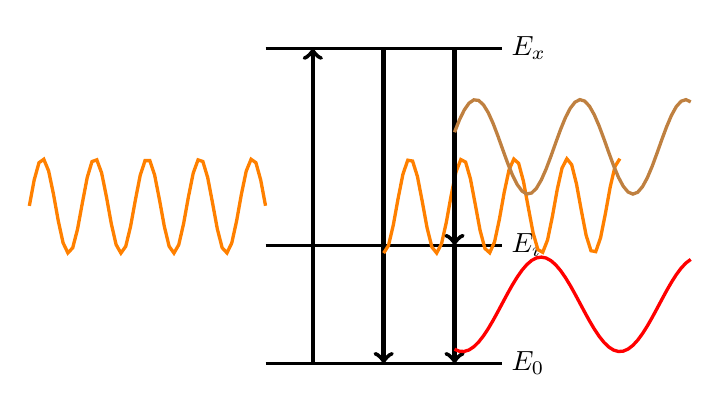
\begin{tikzpicture}
        %%% Definitions
        %% Mathematical constants
        \def \NWAVEFORMSAMPLES {50}

        %% Colors
        \def \INELASTICHIGHCOLOR {brown}
        \def \INELASTICLOWCOLOR {red}

        %% Incoming EM wave
        \def \AMPLITUDE {0.6}
        \def \WAVEFORMLENGTH {3.}
        \def \INWAVESTART {0.}
        \def \INWAVELENGTH {0.5}

        %% Outgoing EM wave
        \def \OUTWAVELENGTHHIGH {1.0}
        \def \OUTWAVELENGTHLOW {1.5}

        %% States
        \def \GROUNDSTATEY {-2.}
        \def \INTERMEDIATESTATEY {-0.5}
        \def \EXCITEDSTATEY {2.}
        \def \STATEXSTART {3.}
        \def \STATEX {3.}

        %% Transitions
        \def \EXCITATIONX {\STATEXSTART+0.2*\STATEX}
        \def \ELASTICX {\STATEXSTART+0.5*\STATEX}
        \def \INELASTICX {\STATEXSTART+0.8*\STATEX}

        %%% Drawing
        %% Incoming EM wave
        \draw [very thick, \ORANGE, domain=\INWAVESTART:\INWAVESTART+\WAVEFORMLENGTH, samples=\NWAVEFORMSAMPLES] plot (\x, {\AMPLITUDE*sin(\WAVEFORMLENGTH/\INWAVELENGTH*2*pi/4*\x r)});

        %% States
        % Ground state
        \draw[very thick, black] (\STATEXSTART, \GROUNDSTATEY) -- (\STATEXSTART+\STATEX, \GROUNDSTATEY);
        \draw (\STATEXSTART + \STATEX, \GROUNDSTATEY) node[anchor=west] {$E_0$};

        % Intermediate state
        \draw[very thick, black] (\STATEXSTART, \INTERMEDIATESTATEY) -- (\STATEXSTART+\STATEX, \INTERMEDIATESTATEY);
        \draw (\STATEXSTART + \STATEX, \INTERMEDIATESTATEY) node[anchor=west] {$E_i$};

        % Excited state
        \draw[very thick, black] (\STATEXSTART, \EXCITEDSTATEY) -- (\STATEXSTART+\STATEX, \EXCITEDSTATEY);
        \draw (\STATEXSTART + \STATEX, \EXCITEDSTATEY) node[anchor=west] {$E_x$};

        %% Transitions
        % Excitation
        \draw[->, ultra thick, black] (\EXCITATIONX, \GROUNDSTATEY) -- (\EXCITATIONX, \EXCITEDSTATEY);

        % Direct ground-state decay
        \visible<2->{
            \draw[->, ultra thick, black] (\ELASTICX, \EXCITEDSTATEY) -- (\ELASTICX, \GROUNDSTATEY);

            \draw [very thick, \ORANGE, domain=\ELASTICX:\ELASTICX+\WAVEFORMLENGTH, samples=\NWAVEFORMSAMPLES] plot (\x, {\AMPLITUDE*sin(\WAVEFORMLENGTH/\INWAVELENGTH*2*pi/4*\x r)});
        }

        % Decay via intermediate states
        \visible<3>{
            \draw[->, ultra thick, black] (\INELASTICX, \EXCITEDSTATEY) -- (\INELASTICX, \INTERMEDIATESTATEY);

            \draw [very thick, \INELASTICHIGHCOLOR, domain=\INELASTICX:\INELASTICX+\WAVEFORMLENGTH, samples=\NWAVEFORMSAMPLES] plot (\x, {\AMPLITUDE*sin(\WAVEFORMLENGTH/\OUTWAVELENGTHHIGH*2*pi/4*\x r) + \INTERMEDIATESTATEY + 0.5*(\EXCITEDSTATEY-\INTERMEDIATESTATEY)});

            \draw[->, ultra thick, black] (\INELASTICX, \INTERMEDIATESTATEY) -- (\INELASTICX, \GROUNDSTATEY);

            \draw [very thick, \INELASTICLOWCOLOR, domain=\INELASTICX:\INELASTICX+\WAVEFORMLENGTH, samples=\NWAVEFORMSAMPLES] plot (\x, {\AMPLITUDE*sin(\WAVEFORMLENGTH/\OUTWAVELENGTHLOW*2*pi/4*\x r) + \GROUNDSTATEY + 0.5*(\INTERMEDIATESTATEY-\GROUNDSTATEY)});
        }
    \end{tikzpicture}
\end{textblock}
\end{frame}

\section{Basics}

\subsection{Resonance Fluorescence in Atoms and Nuclei}

\begin{frame}
    \frametitle{Resonance Fluorescence in Atoms}
    %\begin{textblock}{15.}(0., -4.)
    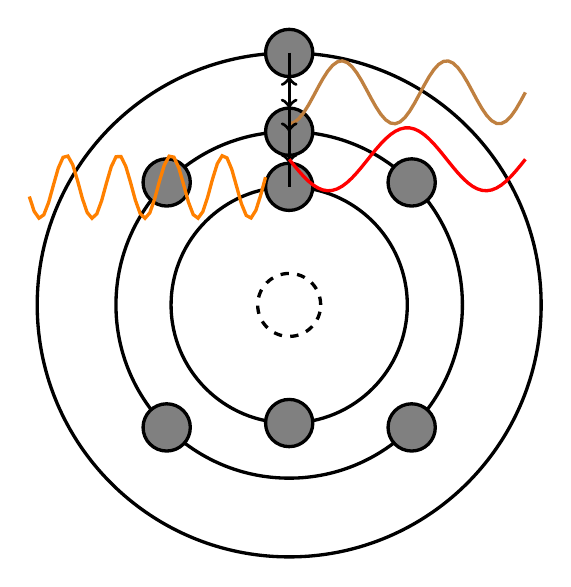
\begin{tikzpicture}
        %%% Definitions
        %% Mathematical constants
        \def \INVERSESQRTTWO {0.7071067811865475}
        \def \NWAVEFORMSAMPLES {50}

        %% Colors
        \def \INELASTICHIGHCOLOR {brown}
        \def \INELASTICLOWCOLOR {red}

        %% Incoming EM wave
        \def \AMPLITUDE {0.4}
        \def \WAVEFORMLENGTH {3.}
        \def \INWAVESTART {0.}
        \def \INWAVELENGTH {0.5}

        %% Outgoing EM wave
        \def \OUTWAVELENGTHHIGH {1.0}
        \def \OUTWAVELENGTHLOW {1.5}

        %% Atom
        \def \ELECTRONRADIUS {0.3}
        \def \ELECTRONCOLOR {gray}

        \def \ORBITALINRADIUS {1.5}
        \def \ORBITALMIDRADIUS {2.2}
        \def \ORBITALOUTRADIUS {3.2}

        \def \ATOMX {5.}
        \coordinate (ATOMPOSITION) at (\ATOMX, 0.);

        %% Nucleus
        \def \NUCLEUSRADIUS {0.4}

        %%% Drawing
        %% Atom
        % Nucleus
        \draw [very thick, black, dashed] (ATOMPOSITION) circle [radius = \NUCLEUSRADIUS];

        % Orbitals
        \draw [very thick, black] (ATOMPOSITION) circle [radius = \ORBITALINRADIUS];
        \draw [very thick, black] (ATOMPOSITION) circle [radius = \ORBITALMIDRADIUS];
        \draw [very thick, black] (ATOMPOSITION) circle [radius = \ORBITALOUTRADIUS];

        % Electrons
        % Inner electrons
        \visible<1-2,5->{
            \draw [very thick, black, fill=\ELECTRONCOLOR] ($ (ATOMPOSITION) + \ORBITALINRADIUS*(0,1)$) circle [radius = \ELECTRONRADIUS];
        }
        \visible<3>{
            \draw [very thick, black, fill=\ELECTRONCOLOR] ($ (ATOMPOSITION) + \ORBITALOUTRADIUS*(0,1)$) circle [radius = \ELECTRONRADIUS];
        }
        \visible<4>{
            \draw [very thick, black, fill=\ELECTRONCOLOR] ($ (ATOMPOSITION) + \ORBITALMIDRADIUS*(0,1)$) circle [radius = \ELECTRONRADIUS];
        }
        \draw [very thick, black, fill=\ELECTRONCOLOR] ($ (ATOMPOSITION) + \ORBITALINRADIUS*(0,-1)$) circle [radius = \ELECTRONRADIUS];

        % Outer electrons
        \draw [very thick, black, fill=\ELECTRONCOLOR] ($ (ATOMPOSITION) + \INVERSESQRTTWO*\ORBITALMIDRADIUS*(1,1)$) circle [radius = \ELECTRONRADIUS];
        \draw [very thick, black, fill=\ELECTRONCOLOR] ($ (ATOMPOSITION) + \INVERSESQRTTWO*\ORBITALMIDRADIUS*(1,-1)$) circle [radius = \ELECTRONRADIUS];
        \draw [very thick, black, fill=\ELECTRONCOLOR] ($ (ATOMPOSITION) + \INVERSESQRTTWO*\ORBITALMIDRADIUS*(-1,1)$) circle [radius = \ELECTRONRADIUS];
        \draw [very thick, black, fill=\ELECTRONCOLOR] ($ (ATOMPOSITION) + \INVERSESQRTTWO*\ORBITALMIDRADIUS*(-1,-1)$) circle [radius = \ELECTRONRADIUS];

        %% Incoming EM wave
        \visible<2>{
            \draw [very thick, \ORANGE, domain=\ATOMX-\ELECTRONRADIUS-\WAVEFORMLENGTH:\ATOMX-\ELECTRONRADIUS, samples=\NWAVEFORMSAMPLES] plot (\x, {\AMPLITUDE*sin(\WAVEFORMLENGTH/\INWAVELENGTH*2*pi/4*\x r) + \ORBITALINRADIUS});
        }

        %% Transitions
        % Excitation
        \visible<3>{
            \draw [->, very thick, black] (\ATOMX, \ORBITALINRADIUS) -- (\ATOMX, \ORBITALOUTRADIUS-\ELECTRONRADIUS);
        }
        \visible<4>{
            \draw [->, very thick, black] (\ATOMX, \ORBITALOUTRADIUS) -- (\ATOMX, \ORBITALMIDRADIUS+\ELECTRONRADIUS);
        }
        \visible<4->{
            \draw [very thick, \INELASTICHIGHCOLOR, domain=\ATOMX:\ATOMX+\WAVEFORMLENGTH, samples=\NWAVEFORMSAMPLES] plot (\x, {\AMPLITUDE*sin(\WAVEFORMLENGTH/\OUTWAVELENGTHHIGH*2*pi/4*\x r) + \ORBITALMIDRADIUS + 0.5*(\ORBITALOUTRADIUS-\ORBITALMIDRADIUS)});
        }
        \visible<5->{
            \draw [->, very thick, black] (\ATOMX, \ORBITALOUTRADIUS) -- (\ATOMX, \ORBITALMIDRADIUS);
            \draw [->, very thick, black] (\ATOMX, \ORBITALMIDRADIUS) -- (\ATOMX, \ORBITALINRADIUS+\ELECTRONRADIUS);
            \draw [very thick, \INELASTICLOWCOLOR, domain=\ATOMX:\ATOMX+\WAVEFORMLENGTH, samples=\NWAVEFORMSAMPLES] plot (\x, {\AMPLITUDE*sin(\WAVEFORMLENGTH/\OUTWAVELENGTHLOW*2*pi/4*\x r) + \ORBITALINRADIUS + 0.5*(\ORBITALMIDRADIUS-\ORBITALINRADIUS)});
        }
    \end{tikzpicture}
\end{textblock}

\begin{textblock}{5.}(8., -6.)
    \begin{center}
        \begin{tabular}{ll}
        & Atom  \\
        \hline
        Res. Energy & $\unit[10^{0}]{eV}$ \\
        Res. Width & $> \unit[10^{-7}]{eV}$ \\
        System mass $\times c^2$ & $\unit[10^{9}]{eV}$ \\
        \end{tabular}
    \end{center}
\end{textblock}

\begin{textblock}{7.}(8.5, -1.5)
    \begin{itemize}
    \visible<2->{
        \item \textbf{Photon source}: \\ 'conventional' light sources, \textbf{laser}
    }
    \visible<6>{
        \item \textbf{Photon spectroscopy}: \\
        prisms, diffraction grids
    }
    \end{itemize}
\end{textblock}

\begin{textblock}{6.}(8.5, 3.2)
    \visible<6>{
        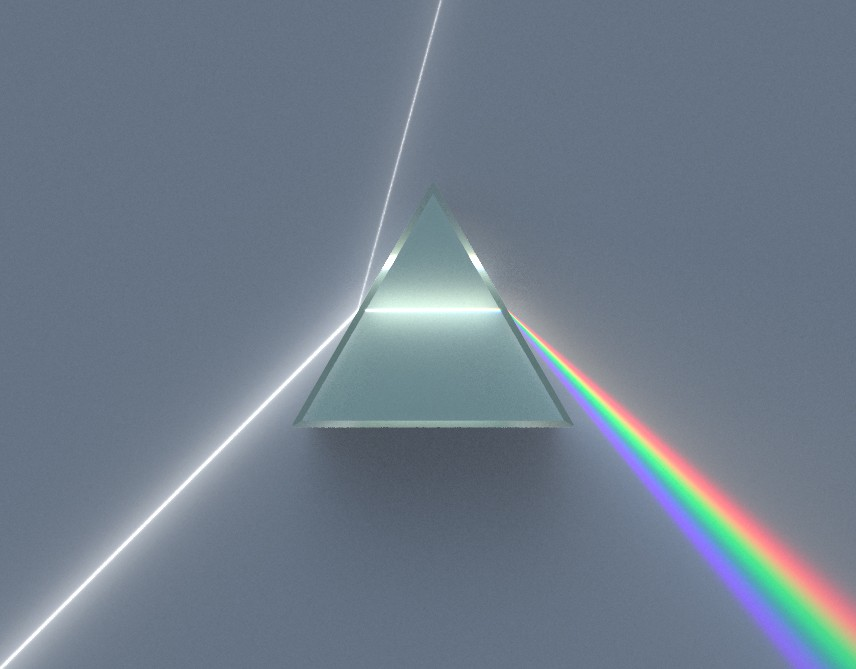
\includegraphics[width=\textwidth]{figures/prism.jpg}
    }
\end{textblock}
\end{frame}

\begin{frame}
    \frametitle{Resonance Fluorescence in Nuclei}
    %    % This file is part of nrf_seminar.

    % nrf_seminar is free software: you can redistribute it and/or modify
    % it under the terms of the GNU General Public License as published by
    % the Free Software Foundation, either version 3 of the License, or
    % (at your option) any later version.

    % nrf_seminar is distributed in the hope that it will be useful,
    % but WITHOUT ANY WARRANTY; without even the implied warranty of
    % MERCHANTABILITY or FITNESS FOR A PARTICULAR PURPOSE.  See the
    % GNU General Public License for more details.

    % You should have received a copy of the GNU General Public License
    % along with nrf_seminar.  If not, see <https://www.gnu.org/licenses/>.

\def \SLIDESTART {1}
\def \SLIDEPHOTONSOURCE {2}
\def \SLIDERADIOACTIVE {3}
\def \SLIDEDECAY {4}
\def \SLIDEEMISSION {5}
\def \SLIDERECOIL {6}
\def \SLIDEWHEEL {7}
\def \SLIDEMOESSBAUER {8}
\def \SLIDEBEAM {9}
\def \SLIDEDETECTION {10}

\begin{textblock}{15.}(0., -3.5)
    \begin{tikzpicture}
        %%% Definitions
        %% Mathematical constants
        \def \NWAVEFORMSAMPLES {50}

        %% Incoming EM wave
        \def \AMPLITUDE {0.4}
        \def \WAVEFORMLENGTH {2.}
        \def \WAVELENGTH {0.4}
        \def \LONGWAVELENGTH {0.6}

        \def \BEAMSTART {0.}
        \def \AMPLITUDEBEAM {0.6}
        \def \WAVEFORMLENGTHBEAM {4.}
        \def \WAVELENGTHBEAMLOW {0.3}
        \def \WAVELENGTHBEAMHIGH {0.5}

        %% Nucleus
        \def \NUCLEUSRADIUS {0.6}

        \def \TARGETNUCLEUSX {5.5}
        \coordinate (TARGETNUCLEUSPOSITION) at (\TARGETNUCLEUSX, 0.);

        \def \SOURCENUCLEUSX {1.5}
        \coordinate (SOURCENUCLEUSPOSITION) at (\SOURCENUCLEUSX, 0.);

        \def \STATEX {2*\NUCLEUSRADIUS}
        \def \MOTHERGROUNDSTATEY {-1.5}
        \def \DAUGHTEREXCITEDSTATEY {-2.2}
        \def \DAUGHTERGROUNDSTATEY {-3.8}

        %% Wheel
        \def \WHEELRADIUS {1.}

        %%% Drawing
        %% Target nucleus
        \visible<-\SLIDEBEAM>{
            \draw [very thick, black, dashed] (TARGETNUCLEUSPOSITION) circle [radius = \NUCLEUSRADIUS];
        }

        % Level scheme of daughter nucleus
        \visible<\SLIDERADIOACTIVE-\SLIDEMOESSBAUER>{
            \draw [very thick, black] (\TARGETNUCLEUSX, \DAUGHTEREXCITEDSTATEY) -- (\TARGETNUCLEUSX + \STATEX, \DAUGHTEREXCITEDSTATEY);
            \draw [very thick, black] (\TARGETNUCLEUSX, \DAUGHTERGROUNDSTATEY) -- (\TARGETNUCLEUSX + \STATEX, \DAUGHTERGROUNDSTATEY);
            \draw (\TARGETNUCLEUSX + 0.5*\STATEX, \DAUGHTERGROUNDSTATEY) node[anchor=north] {$^{57}$Fe};

        %% Source nucleus
            \draw [very thick, black, dashed] (SOURCENUCLEUSPOSITION) circle [radius = \NUCLEUSRADIUS];
        }
        % Recoil direction
        \visible<\SLIDERECOIL>{
            \draw [->, very thick, black] ($ (SOURCENUCLEUSPOSITION) - \NUCLEUSRADIUS*(1.,0.)$) -- ($ (SOURCENUCLEUSPOSITION) - 2*\NUCLEUSRADIUS*(1.,0.)$);
        }

        % Level scheme of mother nucleus
        \visible<\SLIDERADIOACTIVE-\SLIDEMOESSBAUER>{
            \draw [very thick, black] (\SOURCENUCLEUSX - 2*\NUCLEUSRADIUS, \MOTHERGROUNDSTATEY) -- (\SOURCENUCLEUSX - 2*\NUCLEUSRADIUS + \STATEX, \MOTHERGROUNDSTATEY);
            \draw (\SOURCENUCLEUSX + 0.5*\STATEX, \DAUGHTERGROUNDSTATEY) node[anchor=north] {$^{57}$Fe};

        % Level scheme of daughter nucleus
            \draw [very thick, black] (\SOURCENUCLEUSX, \DAUGHTEREXCITEDSTATEY) -- (\SOURCENUCLEUSX + \STATEX, \DAUGHTEREXCITEDSTATEY);
            \draw [very thick, black] (\SOURCENUCLEUSX, \DAUGHTERGROUNDSTATEY) -- (\SOURCENUCLEUSX + \STATEX, \DAUGHTERGROUNDSTATEY);
            \draw (\SOURCENUCLEUSX - 0.5*\STATEX, \DAUGHTERGROUNDSTATEY) node[anchor=north] {$^{57}$Co};
        }

        % Transitions
        % Electron capture
        \visible<\SLIDEDECAY-\SLIDEMOESSBAUER>{
            \draw [->, very thick, black] (\SOURCENUCLEUSX - 0.5*\STATEX, \MOTHERGROUNDSTATEY) -- (\SOURCENUCLEUSX + 0.5*\STATEX, \DAUGHTEREXCITEDSTATEY);
        }
        \visible<\SLIDEEMISSION-\SLIDEMOESSBAUER>{
        % Decay to ground state
            \draw [->, very thick, black] (\SOURCENUCLEUSX + 0.5*\STATEX, \DAUGHTEREXCITEDSTATEY) -- (\SOURCENUCLEUSX + 0.5*\STATEX, \DAUGHTERGROUNDSTATEY);
        
        % Emitted photon
            \draw [very thick, \ORANGE, domain=\SOURCENUCLEUSX+0.5*\STATEX:\SOURCENUCLEUSX+0.5*\STATEX+\WAVEFORMLENGTH, samples=\NWAVEFORMSAMPLES] plot (\x, {\AMPLITUDE*sin(\WAVEFORMLENGTH/\WAVELENGTH*2*pi/4*\x r) + \DAUGHTERGROUNDSTATEY + 0.5*(\DAUGHTEREXCITEDSTATEY - \DAUGHTERGROUNDSTATEY)});
        }
        \visible<\SLIDERECOIL>{
            \draw [very thick, \RED, domain=\SOURCENUCLEUSX+0.5*\STATEX:\SOURCENUCLEUSX+0.5*\STATEX+\WAVEFORMLENGTH, samples=\NWAVEFORMSAMPLES] plot (\x, {\AMPLITUDE*sin(\WAVEFORMLENGTH/\LONGWAVELENGTH*2*pi/4*\x r)});
        }
        \visible<\SLIDEWHEEL-\SLIDEMOESSBAUER>{
            \draw [very thick, \ORANGE, domain=\SOURCENUCLEUSX+0.5*\STATEX:\SOURCENUCLEUSX+0.5*\STATEX+\WAVEFORMLENGTH, samples=\NWAVEFORMSAMPLES] plot (\x, {\AMPLITUDE*sin(\WAVEFORMLENGTH/\WAVELENGTH*2*pi/4*\x r)});
        }

        %% Wheel
        \visible<\SLIDEWHEEL>{
            \draw [very thick, black] ($ (SOURCENUCLEUSPOSITION) + \WHEELRADIUS*(0,1) + \NUCLEUSRADIUS*(0,1)$) circle [radius = \WHEELRADIUS];
            \draw [->, very thick, black] ($ (SOURCENUCLEUSPOSITION) + \WHEELRADIUS*(0,1) + \NUCLEUSRADIUS*(0,1) + 0.5*\WHEELRADIUS*(1., 0.)$) arc [start angle = 0, end angle = 250, radius = 0.5*\WHEELRADIUS];
        }

        \visible<\SLIDEMOESSBAUER>{
            %% Neighboring atoms
            % Top left atom
            \draw [very thick, black, dashed] ($ (SOURCENUCLEUSPOSITION) + 3*\NUCLEUSRADIUS*(0,1)$) circle [radius = \NUCLEUSRADIUS];

            % Top right atom
            \draw [very thick, black, dashed] ($ (SOURCENUCLEUSPOSITION) + 3*\NUCLEUSRADIUS*(1,1)$) circle [radius = \NUCLEUSRADIUS];

            % Bottom right atom
            \draw [very thick, black, dashed] ($ (SOURCENUCLEUSPOSITION) + 3*\NUCLEUSRADIUS*(1,0)$) circle [radius = \NUCLEUSRADIUS];

            % Connection bottom left to top left
            \draw [very thick, black] ($ (SOURCENUCLEUSPOSITION) + \NUCLEUSRADIUS*(0,1)$) -- ($ (SOURCENUCLEUSPOSITION) + 2*\NUCLEUSRADIUS*(0,1)$);

            % Connection top left to top right
            \draw [very thick, black] ($ (SOURCENUCLEUSPOSITION) + 3*\NUCLEUSRADIUS*(0,1) + \NUCLEUSRADIUS*(1,0)$) -- ($ (SOURCENUCLEUSPOSITION) + 3*\NUCLEUSRADIUS*(0,1) + 2*\NUCLEUSRADIUS*(1,0)$);

            % Connection top right to bottom right
            \draw [very thick, black] ($ (SOURCENUCLEUSPOSITION) + 2*\NUCLEUSRADIUS*(0,1) + 3*\NUCLEUSRADIUS*(1,0)$) -- ($ (SOURCENUCLEUSPOSITION) + 1*\NUCLEUSRADIUS*(0,1) + 3*\NUCLEUSRADIUS*(1,0)$);

            % Connection bottom left to bottom right
            \draw [very thick, black] ($ (SOURCENUCLEUSPOSITION) + \NUCLEUSRADIUS*(1,0)$) -- ($ (SOURCENUCLEUSPOSITION) + 2*\NUCLEUSRADIUS*(1,0)$);
        }

        \visible<\SLIDEBEAM>{
            \draw [very thick, \ORANGE, domain=\BEAMSTART:\BEAMSTART+\WAVEFORMLENGTHBEAM, samples=\NWAVEFORMSAMPLES] plot (\x, {\AMPLITUDEBEAM*sin(\WAVEFORMLENGTH/\WAVELENGTH*2*pi/4*\x r)});

            \draw [very thick, \RED, domain=\BEAMSTART:\BEAMSTART+\WAVEFORMLENGTHBEAM, samples=\NWAVEFORMSAMPLES] plot (\x, {\AMPLITUDEBEAM*sin(\WAVEFORMLENGTH/\WAVELENGTHBEAMHIGH*2*pi/4*\x r)});

            \draw [very thick, \YELLOW, domain=\BEAMSTART:\BEAMSTART+\WAVEFORMLENGTHBEAM, samples=\NWAVEFORMSAMPLES] plot (\x, {\AMPLITUDEBEAM*sin(\WAVEFORMLENGTH/\WAVELENGTHBEAMLOW*2*pi/4*\x r)});
        }
    \end{tikzpicture}
\end{textblock}

\begin{textblock}{5.}(7., -6.)
    \begin{center}
        \begin{tabular}{lll}
        & Atom & Nucleus \\
        \hline
        Res. Energy & $\unit[10^{0}]{eV}$ & $\unit[10^{6}]{eV}$ \\
        Res. Width & $\unit[10^{-7}]{eV}$ & $\unit[10^{0}]{eV}$ \\
        System mass $\times c^2$ & $\unit[10^{9}]{eV}$ & $\unit[10^{9}]{eV}$ \\
        \end{tabular}
    \end{center}
\end{textblock}

\begin{textblock}{6.}(8.5, -1.5)
    \begin{itemize}
    \visible<\SLIDEPHOTONSOURCE->{
        \item \textbf{Photon source}: \\ 
        radioactive sources \visible<\SLIDEWHEEL->{[Moon (1951)\visible<\SLIDEMOESSBAUER->{, M\"ossbauer (1958)}]}\visible<\SLIDEBEAM->{, photon beams [Hayward et al. (1957)]}
    }
    \visible<\SLIDEDETECTION>{
        \item \textbf{Photon spectroscopy}: \\
        particle detectors \\(, X-ray diffraction)
    }
    \end{itemize}
\end{textblock}

\begin{textblock}{8.}(0., -5.)
    \visible<\SLIDERECOIL-\SLIDEMOESSBAUER>{
        $\text{relative recoil} \approx \frac{\text{Photon energy}}{\visible<\SLIDEMOESSBAUER>{N \times } \text{Nuclear mass} \times c^2}$
    }
\end{textblock}

\begin{textblock}{6.}(0., -2.)
    \visible<\SLIDEDETECTION>{
        \textit{Realistic image of a gamma-ray detector with some indication of the dimensions.
        I used a picture of two people working on the Gammasphere detectors array, which had been shown in an earlier talk of the series.}
        %\includegraphics[width=\textwidth]{figures/gammasphere.jpg}
    }
\end{textblock}
\end{frame}

\begin{frame}
    \frametitle{Best of two worlds: $^{229m}$Th}
    \begin{textblock}{11.}(2., -4.)
        \includegraphics[width=\textwidth]{figures/th229m.pdf}
    \end{textblock}
\end{frame}

\begin{frame}
    \frametitle{Doppler Broadening}
        % This file is part of nrf_seminar.

    % nrf_seminar is free software: you can redistribute it and/or modify
    % it under the terms of the GNU General Public License as published by
    % the Free Software Foundation, either version 3 of the License, or
    % (at your option) any later version.

    % nrf_seminar is distributed in the hope that it will be useful,
    % but WITHOUT ANY WARRANTY; without even the implied warranty of
    % MERCHANTABILITY or FITNESS FOR A PARTICULAR PURPOSE.  See the
    % GNU General Public License for more details.

    % You should have received a copy of the GNU General Public License
    % along with nrf_seminar.  If not, see <https://www.gnu.org/licenses/>.

\def \SLIDEABSOLUTEZERO {1}
\def \SLIDELN {2}
\def \SLIDEREST {3}
\def \SLIDEROOM {4}
\def \SLIDECRISTAL {5}

\begin{textblock}{9.}(0., -4.)
    \visible<\SLIDEABSOLUTEZERO>{
        \includegraphics[width=\textwidth]{figures/python/cross_section_absolute_zero.pdf}
    }
\end{textblock}
\begin{textblock}{9.}(0., -4.)
    \visible<\SLIDELN-\SLIDEREST>{
        \includegraphics[width=\textwidth]{figures/python/cross_section_ln2.pdf}
    }
\end{textblock}
\begin{textblock}{9.}(0., -4.)
    \visible<\SLIDEROOM>{
        \includegraphics[width=\textwidth]{figures/python/cross_section_room_temperature.pdf}
    }
\end{textblock}
\begin{textblock}{7.}(0., -5.)
    \visible<\SLIDECRISTAL>{
        \includegraphics[width=\textwidth]{figures/crystal_resonance.pdf}
    }
\end{textblock}
\begin{textblock}{7.}(8., 6.)
    \visible<\SLIDECRISTAL>{
        Connection to condensed-matter physics [Lamb, (1939)]
    }
\end{textblock}

\begin{textblock}{8.}(9., -4.)
    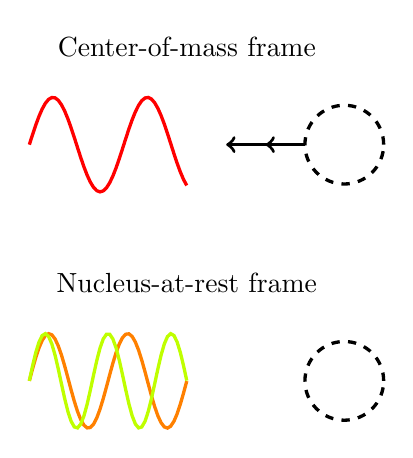
\begin{tikzpicture}
        %%% Definitions
        %% Mathematical constants
        \def \NWAVEFORMSAMPLES {50}

        %% Incoming EM wave
        \def \AMPLITUDE {0.6}
        \def \WAVEFORMLENGTH {2.}
        \def \WAVELENGTH {0.5}
        \def \SHORTWAVELENGTH {0.4}
        \def \LONGWAVELENGTH {0.6}

        %% Inertial frames
        \def \COMY {1.5}
        \def \RESTY {-1.5}
        \def \INERTIALFRAMELABELY {1.}

        %% Nucleus
        \def \NUCLEUSX {4.}
        \coordinate (NUCLEUSCOMPOSITION) at (\NUCLEUSX, \COMY);
        \coordinate (NUCLEUSRESTPOSITION) at (\NUCLEUSX, \RESTY);
        \def \NUCLEUSRADIUS {0.5}

        %%% Drawings
        %% Inertial frame labels
        % COM
        \draw (0.5*\NUCLEUSX, \COMY+\INERTIALFRAMELABELY) node[anchor=south] {Center-of-mass frame};
        % Rest
        \visible<\SLIDEREST->{
            \draw (0.5*\NUCLEUSX, \RESTY+\INERTIALFRAMELABELY) node[anchor=south] {Nucleus-at-rest frame};
        }

        %% Nucleus
        % COM
        \draw [very thick, black, dashed] (NUCLEUSCOMPOSITION) circle [radius=\NUCLEUSRADIUS];
        % Rest
        \visible<\SLIDEREST->{
            \draw [very thick, black, dashed] (NUCLEUSRESTPOSITION) circle [radius=\NUCLEUSRADIUS];
        }

       % Slow movement
        \visible<\SLIDELN-\SLIDEREST>{
            \draw [->, very thick, black] ($ (NUCLEUSCOMPOSITION) - \NUCLEUSRADIUS*(1,0) $) -- ($ (NUCLEUSCOMPOSITION) - 2*\NUCLEUSRADIUS*(1,0) $);
        }
        % Fast movement
        \visible<\SLIDEROOM>{
            \draw [->, very thick, black] ($ (NUCLEUSCOMPOSITION) - \NUCLEUSRADIUS*(1,0) $) -- ($ (NUCLEUSCOMPOSITION) - 3*\NUCLEUSRADIUS*(1,0) $);
        }

        %% Incoming wave
        % COM
        \draw [very thick, \RED, domain=0.:\WAVEFORMLENGTH, samples=\NWAVEFORMSAMPLES] plot (\x, {\AMPLITUDE*sin(\WAVEFORMLENGTH/\LONGWAVELENGTH*2*pi/4*\x r) + \COMY});
        % Rest
        \visible<\SLIDEREST>{
            \draw [very thick, \ORANGE, domain=0.:\WAVEFORMLENGTH, samples=\NWAVEFORMSAMPLES] plot (\x, {\AMPLITUDE*sin(\WAVEFORMLENGTH/\WAVELENGTH*2*pi/4*\x r) + \RESTY});
        }
        \visible<\SLIDEROOM->{
            \draw [very thick, \YELLOW, domain=0.:\WAVEFORMLENGTH, samples=\NWAVEFORMSAMPLES] plot (\x, {\AMPLITUDE*sin(\WAVEFORMLENGTH/\SHORTWAVELENGTH*2*pi/4*\x r) + \RESTY});
        }
    \end{tikzpicture}
\end{textblock}
\end{frame}

\subsection{Experiments}

\begin{frame}
    \frametitle{Absorption or Scattering Spectroscopy?}
    %    % This file is part of nrf_seminar.

    % nrf_seminar is free software: you can redistribute it and/or modify
    % it under the terms of the GNU General Public License as published by
    % the Free Software Foundation, either version 3 of the License, or
    % (at your option) any later version.

    % nrf_seminar is distributed in the hope that it will be useful,
    % but WITHOUT ANY WARRANTY; without even the implied warranty of
    % MERCHANTABILITY or FITNESS FOR A PARTICULAR PURPOSE.  See the
    % GNU General Public License for more details.

    % You should have received a copy of the GNU General Public License
    % along with nrf_seminar.  If not, see <https://www.gnu.org/licenses/>.

\def \SLIDEIN {1}
\def \SLIDETRANS {2}
\def \SLIDENRF {3}
\def \SLIDEDETECTORS {4}
\def \SLIDERESOLUTIONONE {5}
\def \SLIDERESOLUTIONTWO {6}
\def \SLIDERESOLUTIONTHREE {7}
\def \SLIDERESOLUTIONFOUR {8}
\def \SLIDEALTERNATIVERECAP {9}
\def \SLIDEALTERNATIVE {10}
\def \SLIDELASERRED {11}
\def \SLIDELASERORANGE {12}
\def \SLIDELASERGREEN {13}

\begin{textblock}{15.}(0., -5.)
    \begin{tikzpicture}
        %%% Definitions
        %% Mathematical constants
        \def \NWAVEFORMSAMPLES {50}

        %% Incoming EM wave
        \def \AMPLITUDE {0.4}
        \def \WAVEFORMLENGTH {2.5}
        \def \INWAVESTART {0.}
        \def \INREDY {1.5}
        \def \INREDWAVELENGTH {1.4}
        \def \INORANGEY {0.75}
        \def \INORANGEWAVELENGTH {1.2}
        \def \INGREENY {0.}
        \def \INGREENWAVELENGTH {1.0}
        \def \INBLUEY {-0.75}
        \def \INBLUEWAVELENGTH {0.8}
        \def \INVIOLETY {-1.5}
        \def \INVIOLETWAVELENGTH {0.6}

        %% Transmitted EM wave
        \def \TRANSWAVESTART {7.}

        %% Scattered EM wave
        \def \SCATTERINGANGLE {-75}
        \def \SCAWAVEFORMLENGTH {4.}

        %% States
        \def \GROUNDSTATEY {-2.}
        \def \INTERMEDIATESTATEY {-0.5}
        \def \EXCITEDSTATEY {2.}
        \def \STATEXSTART {3.}
        \def \STATEX {3.}

        %% Alternative states
        \def \ALTINTERMEDIATESTATEUPY {0.5}

        %% Transitions
        \def \EXCITATIONX {\STATEXSTART+0.2*\STATEX}
        \def \ELASTICX {\STATEXSTART+0.5*\STATEX}
        \def \INELASTICX {\STATEXSTART+0.8*\STATEX}

        %% Alternative transitions
        \def \ALTEXCITATIONX {\STATEXSTART+0.15*\STATEX}
        \def \ALTELASTICX {\STATEXSTART+0.25*\STATEX}
        \def \ALTEXCITATIONLOWX {\STATEXSTART+0.75*\STATEX}
        \def \ALTDECAYLOWX {\STATEXSTART+0.85*\STATEX}
        \def \ALTEXCITATIONUPX {\STATEXSTART+0.45*\STATEX}
        \def \ALTDECAYUPX {\STATEXSTART+0.55*\STATEX}

        %% Detector
        \def \DETECTORLENGTH {2.}
        \def \DETECTORRADIUS {0.5}
        \def \ABSDETECTORX {10.}
        \def \ABSDETECTORY {0.}
        \def \SCADETECTORX {6.}
        \def \SCADETECTORY {-4.}

        %%% Drawing
        %% Incoming EM waves
        \visible<-\SLIDELASERRED>{
            \draw [very thick, \RED, domain=\INWAVESTART:\INWAVESTART+\WAVEFORMLENGTH, samples=\NWAVEFORMSAMPLES] plot (\x, {\AMPLITUDE*sin(\WAVEFORMLENGTH/\INREDWAVELENGTH*2*pi/4*\x r) + \INREDY});
        }

        \visible<-\SLIDEALTERNATIVE, \SLIDELASERORANGE>{
            \draw [very thick, \ORANGE, domain=\INWAVESTART:\INWAVESTART+\WAVEFORMLENGTH, samples=\NWAVEFORMSAMPLES] plot (\x, {\AMPLITUDE*sin(\WAVEFORMLENGTH/\INORANGEWAVELENGTH*2*pi/4*\x r) + \INORANGEY});
        }

        \visible<-\SLIDEALTERNATIVE, \SLIDELASERGREEN>{
            \draw [very thick, \GREEN, domain=\INWAVESTART:\INWAVESTART+\WAVEFORMLENGTH, samples=\NWAVEFORMSAMPLES] plot (\x, {\AMPLITUDE*sin(\WAVEFORMLENGTH/\INGREENWAVELENGTH*2*pi/4*\x r) + \INGREENY});
        }

        \visible<-\SLIDEALTERNATIVE>{
            \draw [very thick, \BLUE, domain=\INWAVESTART:\INWAVESTART+\WAVEFORMLENGTH, samples=\NWAVEFORMSAMPLES] plot (\x, {\AMPLITUDE*sin(\WAVEFORMLENGTH/\INBLUEWAVELENGTH*2*pi/4*\x r) + \INBLUEY});

            \draw [very thick, \VIOLET, domain=\INWAVESTART:\INWAVESTART+\WAVEFORMLENGTH, samples=\NWAVEFORMSAMPLES] plot (\x, {\AMPLITUDE*sin(\WAVEFORMLENGTH/\INVIOLETWAVELENGTH*2*pi/4*\x r) + \INVIOLETY});
        }

        %% Transmitted EM waves
        \visible<\SLIDETRANS-\SLIDEALTERNATIVERECAP>{
            \draw [very thick, \RED, domain=\TRANSWAVESTART:\TRANSWAVESTART+\WAVEFORMLENGTH, samples=\NWAVEFORMSAMPLES] plot (\x, {\AMPLITUDE*sin(\WAVEFORMLENGTH/\INREDWAVELENGTH*2*pi/4*\x r) + \INREDY});

            \draw [very thick, \ORANGE, domain=\TRANSWAVESTART:\TRANSWAVESTART+\WAVEFORMLENGTH, samples=\NWAVEFORMSAMPLES] plot (\x, {\AMPLITUDE*sin(\WAVEFORMLENGTH/\INORANGEWAVELENGTH*2*pi/4*\x r) + \INORANGEY});
        }
        \visible<\SLIDETRANS-\SLIDEALTERNATIVE>{
            \draw [very thick, \BLUE, domain=\TRANSWAVESTART:\TRANSWAVESTART+\WAVEFORMLENGTH, samples=\NWAVEFORMSAMPLES] plot (\x, {\AMPLITUDE*sin(\WAVEFORMLENGTH/\INBLUEWAVELENGTH*2*pi/4*\x r) + \INBLUEY});

            \draw [very thick, \VIOLET, domain=\TRANSWAVESTART:\TRANSWAVESTART+\WAVEFORMLENGTH, samples=\NWAVEFORMSAMPLES] plot (\x, {\AMPLITUDE*sin(\WAVEFORMLENGTH/\INVIOLETWAVELENGTH*2*pi/4*\x r) + \INVIOLETY});
        }

        %% States
        % Ground state
        \draw[very thick, black] (\STATEXSTART, \GROUNDSTATEY) -- (\STATEXSTART+\STATEX, \GROUNDSTATEY);
        \draw (\STATEXSTART + \STATEX, \GROUNDSTATEY) node[anchor=west] {$E_0$};

        % Intermediate state
        \draw[very thick, black] (\STATEXSTART, \INTERMEDIATESTATEY) -- (\STATEXSTART+\STATEX, \INTERMEDIATESTATEY);
        \draw (\STATEXSTART + \STATEX, \INTERMEDIATESTATEY) node[anchor=west] {$E_i$};

        % Excited state
        \draw[very thick, black] (\STATEXSTART, \EXCITEDSTATEY) -- (\STATEXSTART+\STATEX, \EXCITEDSTATEY);
        \draw (\STATEXSTART + \STATEX, \EXCITEDSTATEY) node[anchor=west] {$E_x$};

        %% Alternative intermediate level
        \visible<\SLIDEALTERNATIVE->{
            \draw[very thick, black] (\STATEXSTART, \ALTINTERMEDIATESTATEUPY) -- (\STATEXSTART+\STATEX, \ALTINTERMEDIATESTATEUPY);
            \draw (\STATEXSTART + \STATEX, \ALTINTERMEDIATESTATEUPY) node[anchor=west] {$E_j$};
        }

        %% Transitions

        \visible<\SLIDETRANS-\SLIDEALTERNATIVERECAP>{    
            % Excitation
            \draw[->, ultra thick, black] (\EXCITATIONX, \GROUNDSTATEY) -- (\EXCITATIONX, \EXCITEDSTATEY);
        }

        \visible<\SLIDENRF-\SLIDEALTERNATIVERECAP>{    
            % Direct ground-state decay
            \draw[->, ultra thick, black] (\ELASTICX, \EXCITEDSTATEY) -- (\ELASTICX, \GROUNDSTATEY);

            \draw [very thick, \GREEN, rotate around={\SCATTERINGANGLE:(\ELASTICX, 0.)}, domain=\ELASTICX:\ELASTICX+\SCAWAVEFORMLENGTH, samples=\NWAVEFORMSAMPLES] plot (\x, {\AMPLITUDE*sin(\SCAWAVEFORMLENGTH/\INORANGEWAVELENGTH*2*pi/4*\x r)});

            % Decay via intermediate states
            \draw[->, ultra thick, black] (\INELASTICX, \EXCITEDSTATEY) -- (\INELASTICX, \INTERMEDIATESTATEY);

            \draw [very thick, \ORANGE, rotate around={\SCATTERINGANGLE:(\INELASTICX, \INTERMEDIATESTATEY + 0.5*(\EXCITEDSTATEY-\INTERMEDIATESTATEY))}, domain=\INELASTICX:\INELASTICX+\SCAWAVEFORMLENGTH, samples=\NWAVEFORMSAMPLES] plot (\x, {\AMPLITUDE*sin(\SCAWAVEFORMLENGTH/\INORANGEWAVELENGTH*2*pi/4*\x r) + \INTERMEDIATESTATEY + 0.5*(\EXCITEDSTATEY-\INTERMEDIATESTATEY)});

            \draw[->, ultra thick, black] (\INELASTICX, \INTERMEDIATESTATEY) -- (\INELASTICX, \GROUNDSTATEY);

            \draw [very thick, \RED, rotate around={\SCATTERINGANGLE:(\INELASTICX, \GROUNDSTATEY + 0.5*(\INTERMEDIATESTATEY-\GROUNDSTATEY))}, domain=\INELASTICX:\INELASTICX+\SCAWAVEFORMLENGTH, samples=\NWAVEFORMSAMPLES] plot (\x, {\AMPLITUDE*sin(\SCAWAVEFORMLENGTH/\INREDWAVELENGTH*2*pi/4*\x r) + \GROUNDSTATEY + 0.5*(\INTERMEDIATESTATEY-\GROUNDSTATEY)});
        }

        %% Alternative decays
        \visible<\SLIDEALTERNATIVE->{
            % Excitation
            \draw[->, ultra thick, black] (\ALTEXCITATIONX, \GROUNDSTATEY) -- (\ALTEXCITATIONX, \EXCITEDSTATEY);
            
            % Direct ground-state decay
            \draw[->, ultra thick, black] (\ALTELASTICX, \EXCITEDSTATEY) -- (\ALTELASTICX, \GROUNDSTATEY);
        }
        \visible<\SLIDEALTERNATIVE, \SLIDELASERGREEN>{
            \draw [very thick, \GREEN, rotate around={\SCATTERINGANGLE:(\ALTELASTICX, 0.)}, domain=\ALTELASTICX:\ALTELASTICX+\SCAWAVEFORMLENGTH, samples=\NWAVEFORMSAMPLES] plot (\x, {\AMPLITUDE*sin(\SCAWAVEFORMLENGTH/\INGREENWAVELENGTH*2*pi/4*\x r)});
        }

        \visible<\SLIDEALTERNATIVE->{
            % Excitation and decay of upper intermediate state
            \draw[->, ultra thick, black] (\ALTEXCITATIONUPX, \GROUNDSTATEY) -- (\ALTEXCITATIONUPX, \ALTINTERMEDIATESTATEUPY);

            \draw[->, ultra thick, black] (\ALTDECAYUPX, \GROUNDSTATEY) -- (\ALTDECAYUPX, \ALTINTERMEDIATESTATEUPY);
        }
        \visible<\SLIDEALTERNATIVE, \SLIDELASERORANGE>{
            \draw [very thick, \ORANGE, rotate around={\SCATTERINGANGLE:(\ALTDECAYUPX, \GROUNDSTATEY + 0.5*(\ALTINTERMEDIATESTATEUPY-\GROUNDSTATEY))}, domain=\ALTDECAYUPX:\ALTDECAYUPX+\SCAWAVEFORMLENGTH, samples=\NWAVEFORMSAMPLES] plot (\x, {\AMPLITUDE*sin(\SCAWAVEFORMLENGTH/\INORANGEWAVELENGTH*2*pi/4*\x r) + \GROUNDSTATEY + 0.5*(\ALTINTERMEDIATESTATEUPY-\GROUNDSTATEY)});
        }

        \visible<\SLIDEALTERNATIVE->{
            % Excitation and decay of upper intermediate state
            \draw[->, ultra thick, black] (\ALTEXCITATIONLOWX, \INTERMEDIATESTATEY) -- (\ALTEXCITATIONLOWX, \GROUNDSTATEY);

            \draw[->, ultra thick, black] (\ALTDECAYLOWX, \INTERMEDIATESTATEY) -- (\ALTDECAYLOWX, \GROUNDSTATEY);
        }
        \visible<\SLIDEALTERNATIVE, \SLIDELASERRED>{
            \draw [very thick, \RED, rotate around={\SCATTERINGANGLE:(\ALTDECAYLOWX, \GROUNDSTATEY + 0.5*(\INTERMEDIATESTATEY-\GROUNDSTATEY))}, domain=\ALTDECAYLOWX:\ALTDECAYLOWX+\SCAWAVEFORMLENGTH, samples=\NWAVEFORMSAMPLES] plot (\x, {\AMPLITUDE*sin(\SCAWAVEFORMLENGTH/\INREDWAVELENGTH*2*pi/4*\x r) + \GROUNDSTATEY + 0.5*(\INTERMEDIATESTATEY-\GROUNDSTATEY)});
        }

        \visible<\SLIDEDETECTORS->{
                %% Absorption detector
                \visible<-\SLIDEALTERNATIVE>{
                \draw[very thick, black, fill=gray]     (\ABSDETECTORX, \ABSDETECTORY) 
                -- (\ABSDETECTORX, \ABSDETECTORY + \DETECTORRADIUS)
                -- (\ABSDETECTORX + \DETECTORLENGTH, \ABSDETECTORY + \DETECTORRADIUS)
                -- (\ABSDETECTORX + \DETECTORLENGTH, \ABSDETECTORY - \DETECTORRADIUS)
                -- (\ABSDETECTORX, \ABSDETECTORY - \DETECTORRADIUS)
                -- (\ABSDETECTORX, \ABSDETECTORY);
            }

            %% Scattering detector
            \draw[very thick, black, rotate around={\SCATTERINGANGLE:(\SCADETECTORX, \SCADETECTORY)}, fill=gray]     (\SCADETECTORX, \SCADETECTORY) 
            -- (\SCADETECTORX, \SCADETECTORY + \DETECTORRADIUS)
            -- (\SCADETECTORX + \DETECTORLENGTH, \SCADETECTORY + \DETECTORRADIUS)
            -- (\SCADETECTORX + \DETECTORLENGTH, \SCADETECTORY - \DETECTORRADIUS)
            -- (\SCADETECTORX, \SCADETECTORY - \DETECTORRADIUS)
            -- (\SCADETECTORX, \SCADETECTORY);
        }
    \end{tikzpicture}
\end{textblock}

\def \SPECTRUMWIDTH {5.5}
\def \SPECTRUMY {2.6}
\def \SCASPECTRUMX {0.}
\def \TRASPECTRUMX {9.5}

\visible<\SLIDERESOLUTIONONE, \SLIDEALTERNATIVERECAP>{
    \begin{textblock}{\SPECTRUMWIDTH}(\SCASPECTRUMX, \SPECTRUMY)
        \includegraphics[width=\textwidth]{figures/python/scattering_001.pdf}
    \end{textblock}

    \begin{textblock}{\SPECTRUMWIDTH}(\TRASPECTRUMX, \SPECTRUMY)
        \includegraphics[width=\textwidth]{figures/python/transmission_001.pdf}
    \end{textblock}
}

\visible<\SLIDERESOLUTIONTWO>{
    \begin{textblock}{\SPECTRUMWIDTH}(\SCASPECTRUMX, \SPECTRUMY)
        \includegraphics[width=\textwidth]{figures/python/scattering_005.pdf}
    \end{textblock}

    \begin{textblock}{\SPECTRUMWIDTH}(\TRASPECTRUMX, \SPECTRUMY)
        \includegraphics[width=\textwidth]{figures/python/transmission_005.pdf}
    \end{textblock}
}

\visible<\SLIDERESOLUTIONTHREE>{
    \begin{textblock}{\SPECTRUMWIDTH}(\SCASPECTRUMX, \SPECTRUMY)
        \includegraphics[width=\textwidth]{figures/python/scattering_01.pdf}
    \end{textblock}

    \begin{textblock}{\SPECTRUMWIDTH}(\TRASPECTRUMX, \SPECTRUMY)
        \includegraphics[width=\textwidth]{figures/python/transmission_01.pdf}
    \end{textblock}
}

\visible<\SLIDERESOLUTIONFOUR>{
    \begin{textblock}{\SPECTRUMWIDTH}(\SCASPECTRUMX, \SPECTRUMY)
        \includegraphics[width=\textwidth]{figures/python/scattering_03.pdf}
    \end{textblock}

    \begin{textblock}{\SPECTRUMWIDTH}(\TRASPECTRUMX, \SPECTRUMY)
        \includegraphics[width=\textwidth]{figures/python/transmission_03.pdf}
    \end{textblock}
}

\visible<\SLIDEALTERNATIVE>{
    \begin{textblock}{\SPECTRUMWIDTH}(\SCASPECTRUMX, \SPECTRUMY)
        \includegraphics[width=\textwidth]{figures/python/scattering_001.pdf}
    \end{textblock}

    \begin{textblock}{\SPECTRUMWIDTH}(\TRASPECTRUMX, \SPECTRUMY)
        \includegraphics[width=\textwidth]{figures/python/transmission_alternative_001.pdf}
    \end{textblock}
}

\visible<\SLIDELASERRED>{
    \begin{textblock}{\SPECTRUMWIDTH}(\SCASPECTRUMX, \SPECTRUMY)
        \includegraphics[width=\textwidth]{figures/python/scattering_single_0_001.pdf}
    \end{textblock}    
}

\visible<\SLIDELASERORANGE>{
    \begin{textblock}{\SPECTRUMWIDTH}(\SCASPECTRUMX, \SPECTRUMY)
        \includegraphics[width=\textwidth]{figures/python/scattering_single_1_001.pdf}
    \end{textblock}    
}

\visible<\SLIDELASERGREEN>{
    \begin{textblock}{\SPECTRUMWIDTH}(\SCASPECTRUMX, \SPECTRUMY)
        \includegraphics[width=\textwidth]{figures/python/scattering_single_2_001.pdf}
    \end{textblock}    
}
\end{frame}

\subsection{Photon Sources}

\begin{frame}
    \frametitle{Bremsstrahlung}
        % This file is part of nrf_seminar.

    % nrf_seminar is free software: you can redistribute it and/or modify
    % it under the terms of the GNU General Public License as published by
    % the Free Software Foundation, either version 3 of the License, or
    % (at your option) any later version.

    % nrf_seminar is distributed in the hope that it will be useful,
    % but WITHOUT ANY WARRANTY; without even the implied warranty of
    % MERCHANTABILITY or FITNESS FOR A PARTICULAR PURPOSE.  See the
    % GNU General Public License for more details.

    % You should have received a copy of the GNU General Public License
    % along with nrf_seminar.  If not, see <https://www.gnu.org/licenses/>.

\begin{textblock}{8.}(0., -4.)
    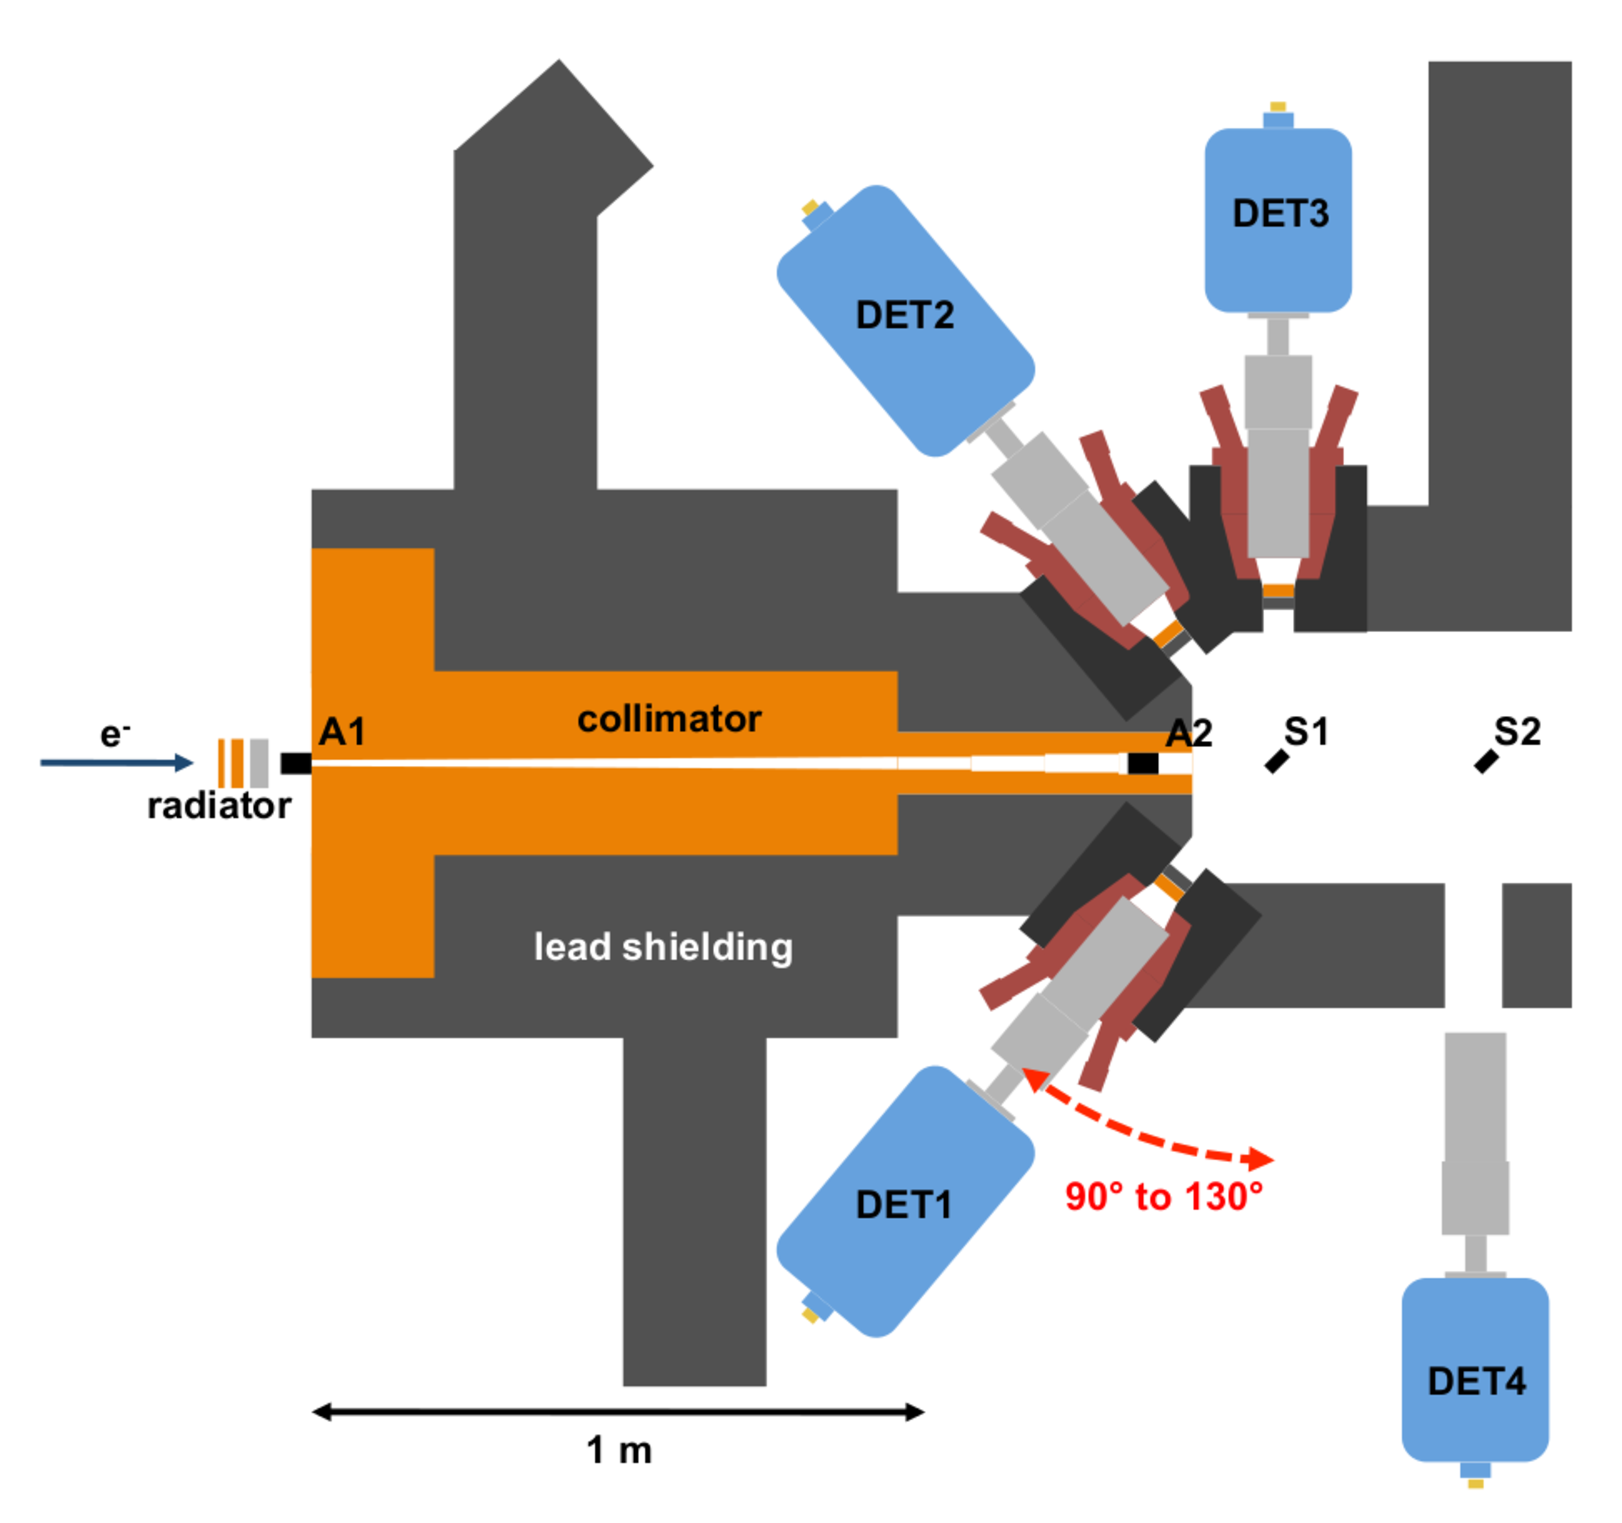
\includegraphics[width=\textwidth]{figures/dhips.pdf}
\end{textblock}

\begin{textblock}{6.}(9., -5.)
    \begin{itemize}
        \item Hayward et al. (1957)
        \item Continuous spectrum of photons up to the maximum electron energy
    \end{itemize}
\end{textblock}

\def \SPECTRUMX {9.}
\def \SPECTRUMY {0.}

\begin{textblock}{6.}(\SPECTRUMX, \SPECTRUMY)
    \visible<2>{
        \includegraphics[width=\textwidth]{figures/python/bremsstrahlung_linear.pdf}
    }
\end{textblock}

\begin{textblock}{6.}(\SPECTRUMX, \SPECTRUMY)
    \visible<3>{
        \includegraphics[width=\textwidth]{figures/python/bremsstrahlung_logarithmic.pdf}
    }
\end{textblock}
\end{frame}

\begin{frame}
    \frametitle{Quasimonochromatic (Polarized) Photon Beams}
    \begin{textblock}{9.}(0., -4.)
    \includegraphics[width=\textwidth]{figures/higs.pdf}
\end{textblock}

\begin{textblock}{6.}(9., -5.)
    \begin{itemize}
        \item Pietralla, Ahmed et al. (2002)
        \item Quasi-monochromatic spectrum of photons with tunable energy
        \item High polarization
    \end{itemize}
\end{textblock}

\def \SPECTRUMX {9.}
\def \SPECTRUMY {1.}

\begin{textblock}{6.}(\SPECTRUMX, \SPECTRUMY)
    \includegraphics[width=\textwidth]{figures/python/quasimonochromatic.pdf}
\end{textblock}

\begin{textblock}{6.}(1., 3.)
    \visible<2>{
        \begin{itemize}
            \item European effort
        \end{itemize}
        \includegraphics[width=\textwidth]{figures/eli_np_logo.png}
    }
\end{textblock}
\end{frame}

\begin{frame}
    \frametitle{Spectrum}
    \begin{textblock}{9.5}(0., -4.)
    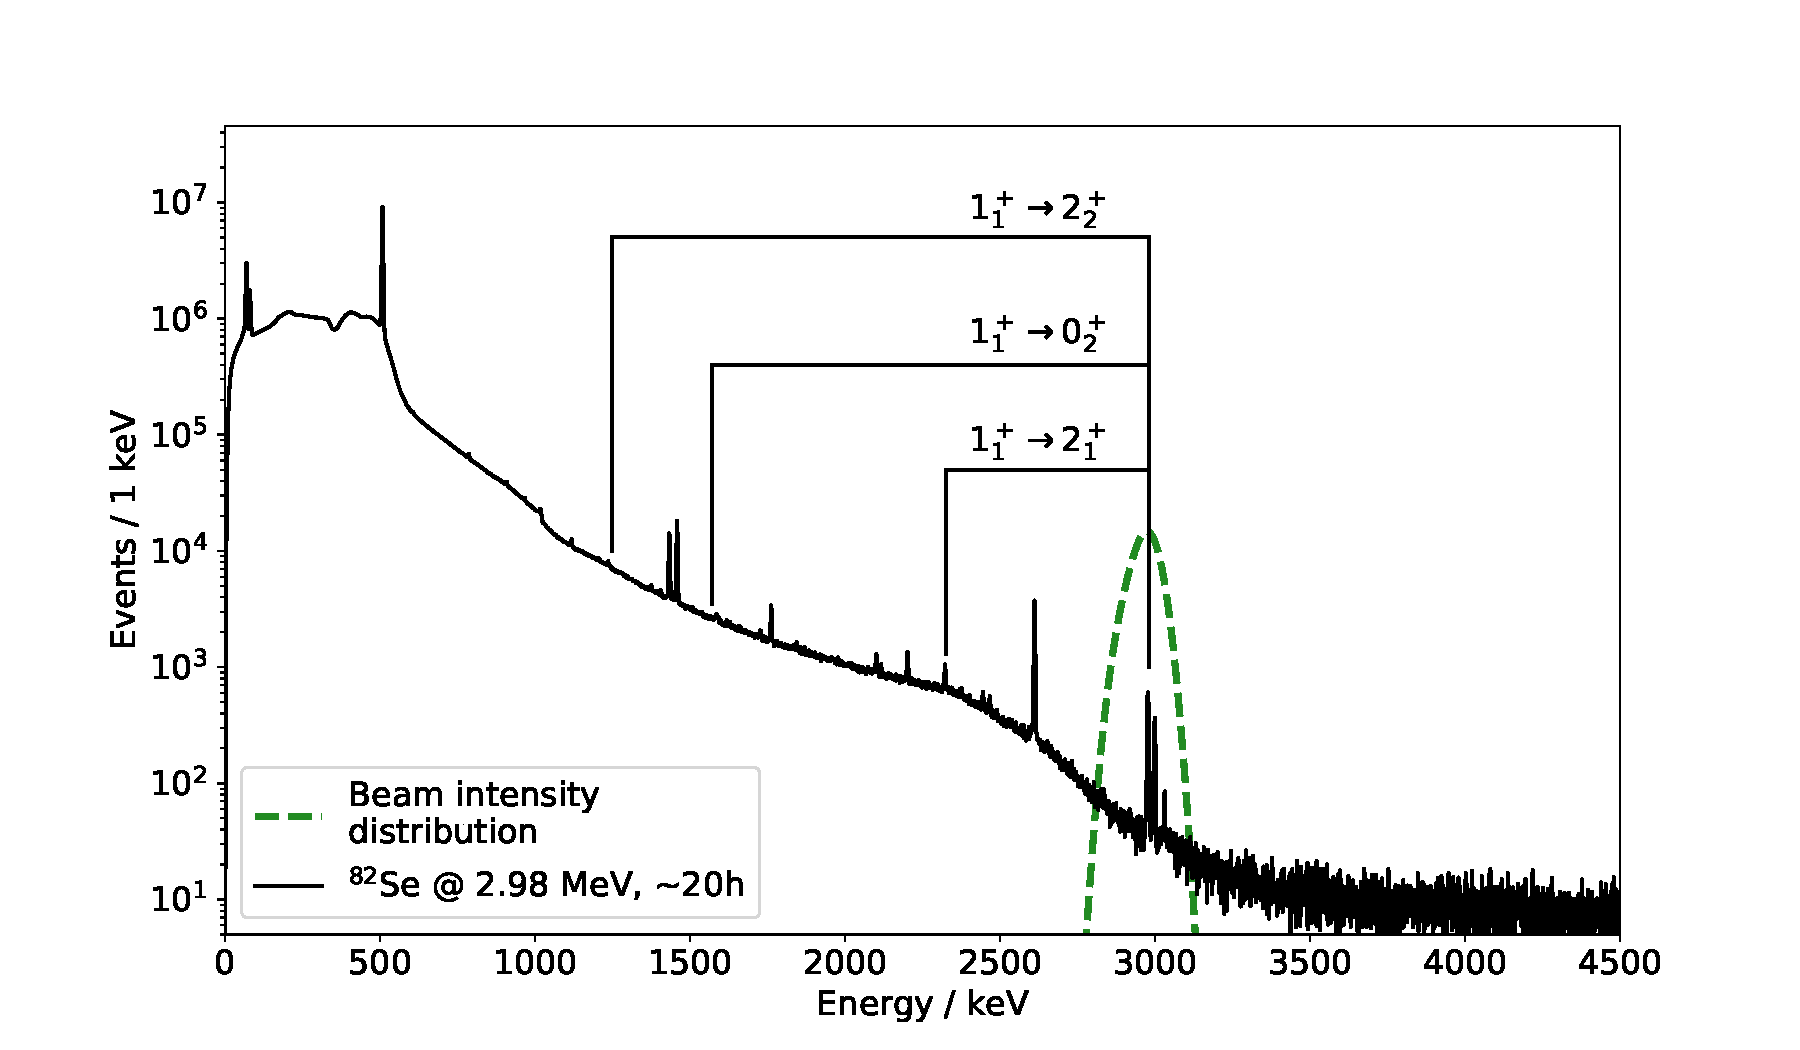
\includegraphics[width=\textwidth, trim=50 0 50 50,clip]{figures/se82_spectrum_branchings.pdf}
\end{textblock}

\begin{textblock}{5.}(10., -5)
    \color{green}\textbf{Advantages} \color{black} of the NRF technique
    \begin{itemize}
        \item Model-independent
        \item High resolution
        \item (Selectivity)
    \end{itemize}
    
    \color{red}\textbf{Disadvantages}\color{black}
    \begin{itemize}
        \item Nonresonant background
        \item Low cross section (long experiments, large samples, stable isotopes)
        \item Inefficient detection
    \end{itemize}
\end{textblock}
\end{frame}

\section{Applications}

\subsection{Fundamental Research}

\begin{frame}
    \frametitle{r-Process Nucleosynthesis}
        % This file is part of nrf_seminar.

    % nrf_seminar is free software: you can redistribute it and/or modify
    % it under the terms of the GNU General Public License as published by
    % the Free Software Foundation, either version 3 of the License, or
    % (at your option) any later version.

    % nrf_seminar is distributed in the hope that it will be useful,
    % but WITHOUT ANY WARRANTY; without even the implied warranty of
    % MERCHANTABILITY or FITNESS FOR A PARTICULAR PURPOSE.  See the
    % GNU General Public License for more details.

    % You should have received a copy of the GNU General Public License
    % along with nrf_seminar.  If not, see <https://www.gnu.org/licenses/>.

\begin{textblock}{7.}(0., -4.)
    \begin{itemize}
        \item Synthesis of heavy elements in the universe
        \item Competition between photoabsorption (photodisintegration) and neutron capture
    \end{itemize}
\end{textblock}

\begin{textblock}{9.}(0., 3.)
    \textit{Schematic figure that shows the competition between neutron capture and photodisintegration in the r-process.
    I chose a figure from a textbook by C. Iliadis.}
    %\includegraphics[width=\textwidth]{figures/r_process_schematic.pdf}
\end{textblock}

\begin{textblock}{7.}(8., -4.)
    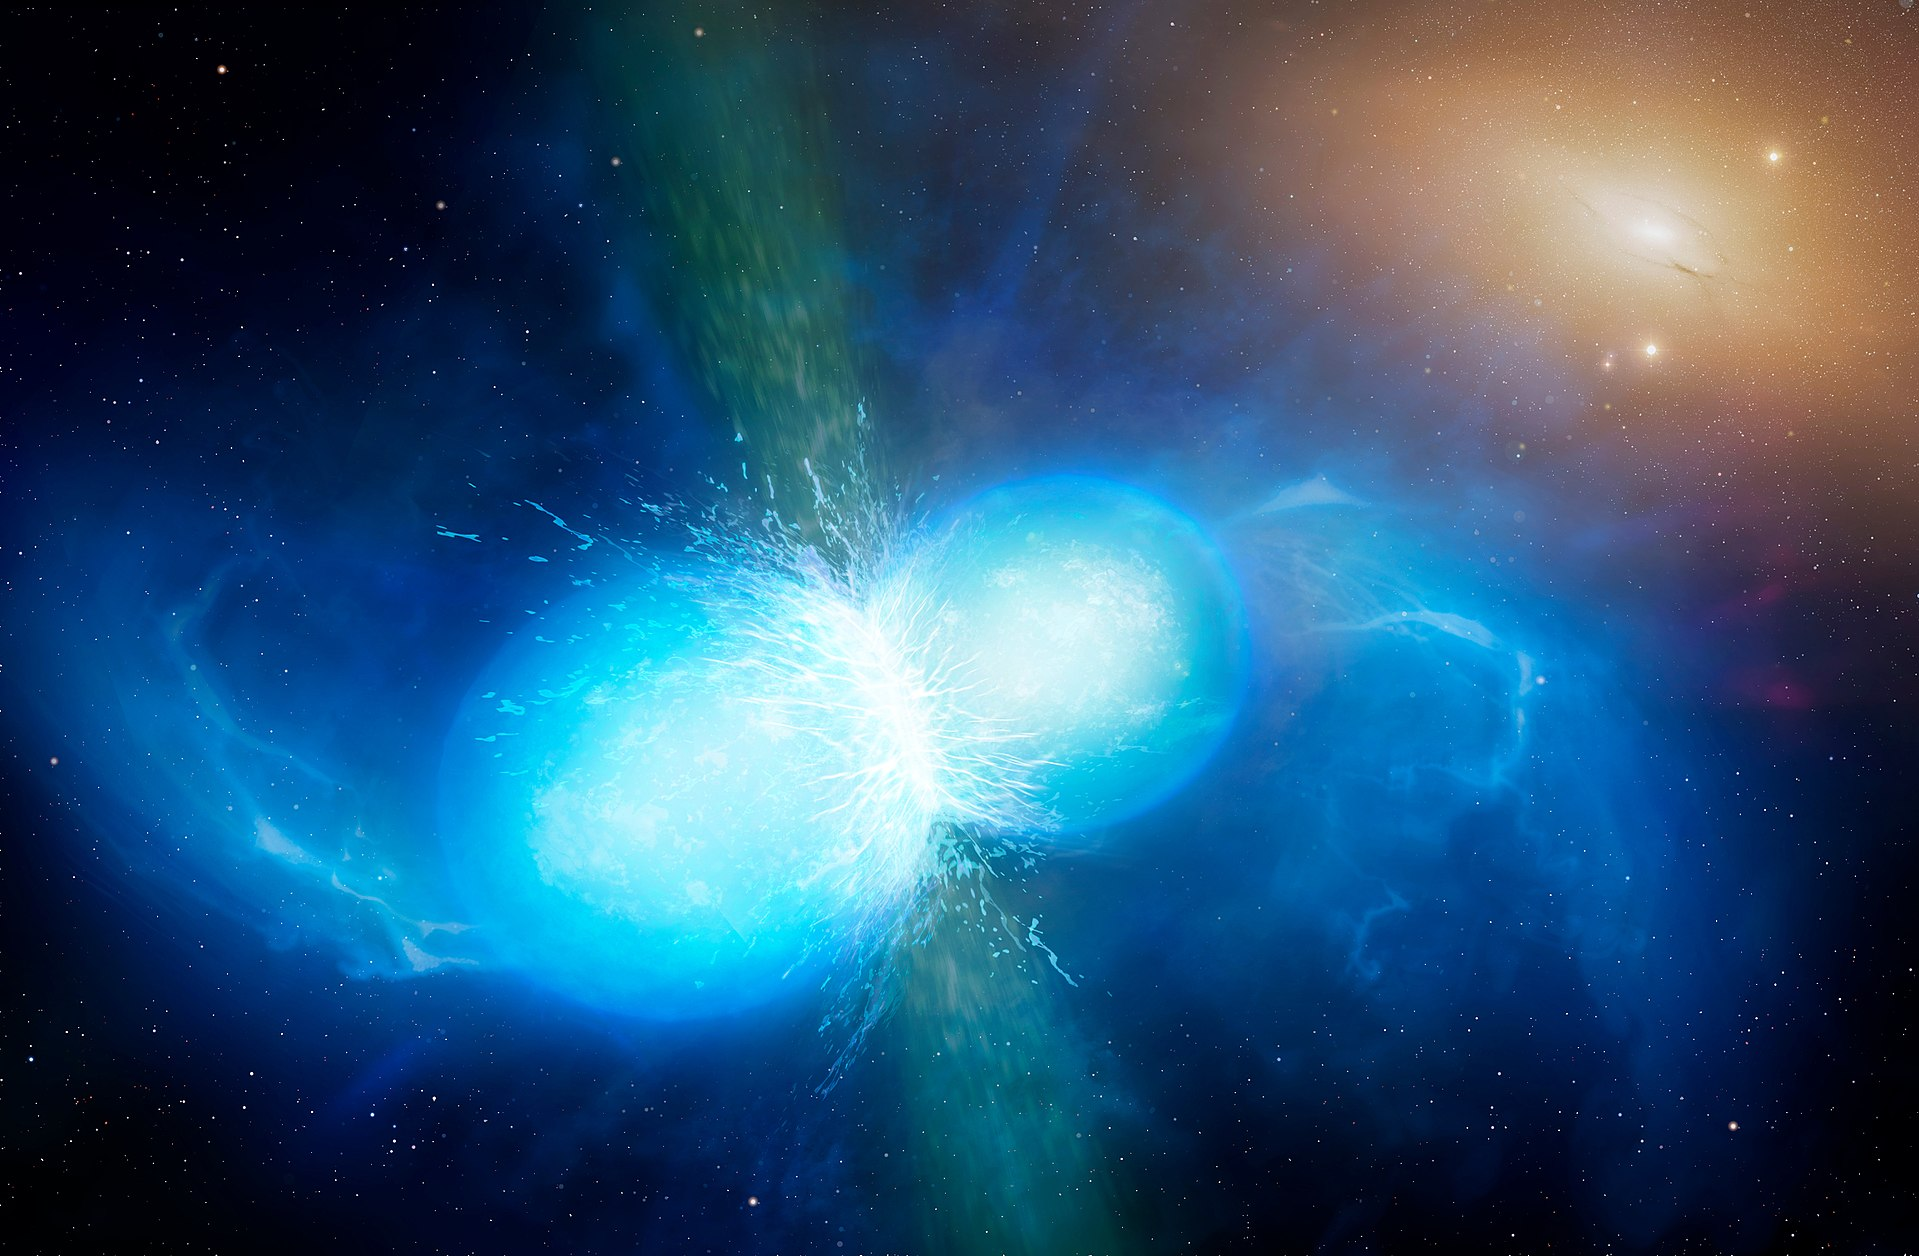
\includegraphics[width=\textwidth]{figures/neutron_star_merger.jpg}
\end{textblock}  
\end{frame}

\subsection{Technical Applications}

\begin{frame}
    \frametitle{Isotope-selective Scanning}
        % This file is part of nrf_seminar.

    % nrf_seminar is free software: you can redistribute it and/or modify
    % it under the terms of the GNU General Public License as published by
    % the Free Software Foundation, either version 3 of the License, or
    % (at your option) any later version.

    % nrf_seminar is distributed in the hope that it will be useful,
    % but WITHOUT ANY WARRANTY; without even the implied warranty of
    % MERCHANTABILITY or FITNESS FOR A PARTICULAR PURPOSE.  See the
    % GNU General Public License for more details.

    % You should have received a copy of the GNU General Public License
    % along with nrf_seminar.  If not, see <https://www.gnu.org/licenses/>.

\begin{textblock}{9.}(0., -4.)
    \includegraphics[width=\textwidth]{figures/snm.pdf}
\end{textblock}

\begin{textblock}{7.}(8., -2.)
    \begin{itemize}
        \item Narrow nuclear resonances $\to$ high sensitivity to isotopic composition
        \item Non-destructive and highly penetrative
    \end{itemize}
\end{textblock}
\end{frame}

\begin{frame}
    \frametitle{References}
    \begin{textblock}{15.}(0., -5.)
    \begin{itemize}
        \item Prism: \url{https://de.wikipedia.org/wiki/Prisma_(Optik)}
        \item Gammasphere: \url{https://www.phy.anl.gov/gammasphere/}
        \item $^{229m}$Th: L. von der Wense et al., Nature \textbf{533} (2016) 47-51
        \item Resonance shape for a crystal: W. E. Lamb, Phys. Rev. \textbf{55} (1939) 190-197
        \item DHIPS: C. Romig, Dissertation, Technische Universit\"at Darmstadt (2015)
        \item HI$\gamma$S: H. R. Weller et al., Prog. Part. Nucl. Phys. \textbf{62} (2009) 257-303
        \item Spectrum: U. Friman-Gayer, Dissertation, Technische Universit\"at Darmstadt (2020)
        \item Schematic r-Process: C. Iliadis, Nuclear Physics of Stars, Wiley-VCH (2015)
        \item Neutron star merger: \url{https://en.wikipedia.org/wiki/Neutron_star_merger}
    \end{itemize}
    \end{textblock}
\end{frame}

\end{document}